\documentclass[a4paper, twoside, 11pt]{article}
% It is needed to use this command for automatic compilation in VSCode
% !TEX program = lualatexmk

%DOCUMENT, PREAMBLE AND MACROS DESIGNED FOR LuaLaTeX%
\newcommand{\fbar}{\FloatBarrier}

\usepackage{amsmath} %matematic package%
\usepackage{textcomp} %for miscellaneous symbols%
%\usepackage{times} %times font%
\usepackage{graphicx} %enhanced support for craphics%
%\usepackage{mathptmx} %use Times as default text font, and provide maths support%
\usepackage{cmap} %mapování znaků - vyhledávání v pdf%
\usepackage[czech]{babel}%CZ%
\usepackage[utf8]{inputenc}%kódování%
\usepackage[T1]{fontenc}%kódování%
\usepackage{multirow}%Multirow table support
\usepackage{float}%Improves the interface for defining floating objects such as figures and tables%
\usepackage{wasysym} %for various glyphs, symbols%

\usepackage{setspace}%spacing% 
\onehalfspacing

\usepackage{hyperref}
\hypersetup{
    colorlinks=true, %pokud nechci definovat citecolor=black aby byly odkazy citací černé, tak dám colorlinks=false,%
    bookmarks=true,
    linkcolor=black,
    citecolor=black,
    urlcolor=black,
}

%when using LuaLaTex, defining Times Fonts from your system - it has to be named like this and inserted ttf file in the folder of your tex file%
\usepackage{fontspec}
\selectlanguage{czech}
\setmainfont[Ligatures=TeX,BoldFont={* Bold}] {Times New Roman}
                                
\setsansfont[Ligatures=TeX,BoldFont={* Bold}]{Times New Roman}
                                      
\setmonofont{Times New Roman}
 
%\usepackage[italic]{mathastext} %for text in math environment, better looking times then



%for CITATIONS URL to work, it is not needed when you are not using URL label%
\usepackage{url}
\usepackage{csquotes}
\usepackage[style=iso-numeric, backend=biber, isbn=true, urldate=iso,seconds=true, date=terse, datezeros=true, language=czech]{biblatex}
\addbibresource{src/bib/zdroje.bib} % BIB resources to import
%\DeclareUrlCommand\url{\def\UrlLeft{<}\def\UrlRight{>} \urlstyle{tt}}



%\usepackage{biblatex}
%END for citations%

%changing bibliography font%
\renewcommand*{\bibfont}{\fontspec{Times New Roman}}

\usepackage{comment} %For comments%
\usepackage{pdfpages}%for pdf pages%
\usepackage{enumerate}%For lists%
\usepackage{enumitem}%For Custom Numbering Nested Lists%
\setlist[enumerate]{label*=\arabic*.} %setting Number. numbering in lists%
\usepackage{tikz} %For vector graphics%
\usepackage{circuitikz}%For schemes%
\usepackage{pgf} %Post script graphics for tikz%

%pouze funguje v PDFLaTeX%
%\usepackage{tgtermes}%na times font, jiný nefunguje s vyhledáváním a copy%

%
\usepackage{placeins}%% for \FloatBarrier command that blocks floating with htbp! go over \FloatBarrier
\usepackage{mathrsfs}%packagee for math symbols for Laplace, Z transform etc., usage \mathscr{Z}
\usepackage{upgreek}%for upgreek symbols, specified tau \uptau

%this works only when using PDFLaTeX%
\usepackage[list=true,listformat=simple]{subcaption}
\usepackage[figurename=Obr.,font=small,labelfont=it,textfont=it]{caption} %for renaming figures instead of renewcommand, small for 11pt default is 10pt as needed in word template
\usepackage[tablename=Tab.,font=small,labelfont=it,
            textfont=it]{caption} %for renaming tables instead of renewcommand
            

            %this works with LuaLaTex and fontspec package%
 \DeclareCaptionFont{times}{\fontspec{Times New Roman Italic}}

%labelfont and textfont defined here only works with previous declarecaptionfont times and fontspec%
\captionsetup{labelfont=times, textfont=times, labelsep=space}%no separator in captions
%

%\bibliographystyle{czechiso} %czechiso.bst in folder is needed for this style to work, available at http://www.fit.vutbr.cz/~martinek/latex/czechiso.html%

%\hyperref[label]{text}% Help for targeting labels

\usepackage{chngcntr} %for numbered figures with sections
\usepackage{tocloft}%better TOC

%\usepackage{a4wide}%širší a4%
\usepackage[inner=3cm,outer=2cm,top=2.5cm,bottom=2.5cm,footskip=1cm]{geometry}%for propper margins
\usepackage{textcase}%for making text uppercase without caps \MakeTextUppercase
 
 
\usepackage{titlesec}%for spacing text after sections
\usepackage{parskip}[]%for working \parskip
\newcommand{\sectionbreak}{\clearpage}%maybe for SECTIONS on a new page

\usepackage[titletoc]{appendix}%For appendix - přílohy, titletoc is crucial
%\renewcommand{\appendixname}{Příloha}

\setlength{\parindent}{0.5cm}%setting indent of paragraph to 0.5cm
\setlength{\parskip}{0em}%setting parskip to 0 for \titleformat to work properly with parskip package

\usepackage{colortbl}%for colored cells
\usepackage{xcolor}%for colors
\definecolor{ctublue}{HTML}{0065BD}%defining ctu color
\definecolor{ctugreen}{HTML}{A2AD00}
\definecolor{ctured}{HTML}{C60C30}
\definecolor{ctuyellow}{HTML}{F0AB00}
\definecolor{ctugreenyblue}{HTML}{00B2A9}
\definecolor{ctulightblue}{HTML}{6AADE4}
\definecolor{ctuorange}{HTML}{E05206}
\definecolor{lightgray}{HTML}{D1D5DB}


\titlespacing*{\section}{0em}{1em}{-\parskip}%spacing text after sections from titlesec package
\titlespacing*{\subsection}{0em}{1em}{-\parskip}%spacing text after sections from titlesec package
\titlespacing*{\subsubsection}{0em}{1em}{-\parskip}%spacing text after sections from titlesec package

%when you want sectin/sub/subsub to be black, delete \color{ctublue}
\titleformat{\section}{\color{ctublue}\fontspec{Times New Roman}\fontsize{15}{15}\bfseries}{\thesection}{2.1em}{}%defining title sizes by word template
\titleformat{\subsection}{\color{ctublue}\fontspec{Times New Roman}\fontsize{14}{14}\bfseries}{\thesubsection}{1.53em}{}%defining title sizes by word template
\titleformat{\subsubsection}{\color{ctublue}\fontspec{Times New Roman}\fontsize{13}{13}\bfseries}{\thesubsubsection}{1em}{}%defining title sizes by word template


\usepackage{ctable}%imports xtable with booktabs
\usepackage{multicol}

\usepackage{listings}%for code environments - \begin{lstlisting}


\definecolor{codegreen}{rgb}{0,0.6,0}
\definecolor{codegray}{rgb}{0.5,0.5,0.5}
\definecolor{codepurple}{rgb}{0.58,0,0.82}
\definecolor{backcolour}{rgb}{0.95,0.95,0.92}


\lstdefinestyle{zakopal}{
    backgroundcolor=\color{lightgray},   
    commentstyle=\color{white},
    keywordstyle=\color{magenta},
    numberstyle=\tiny\color{codegray},
    stringstyle=\color{codepurple},
    basicstyle=\ttfamily\footnotesize,
    breakatwhitespace=false,         
    breaklines=true,                 
    captionpos=b,                    
    keepspaces=true,                 
    numbers=left,                    
    numbersep=5pt,                  
    showspaces=false,                
    showstringspaces=false,
    showtabs=false,                  
    tabsize=2
}
\lstset{style=zakopal}
\renewcommand{\lstlistingname}{Kód}% renaming Listing -> Kód 
\renewcommand{\lstlistlistingname}{Seznam kódů}% renaming List of Listings -> Seznam kódů

\lstdefinelanguage{SCL}
{morekeywords={FUNCTION_BLOCK,BEGIN,NOT,END_FUNCTION_BLOCK,FUNCTION,VOID,VAR_INPUT,END_VAR,VAR_IN_OUT,IF,
THEN,END_IF,END_FUNCTION,BOOL,FALSE,TRUE},
sensitive=false,
morecomment=[l]{//},
morestring=[b]",
literate={;}{{\textcolor{orange}{;}}}{1}
{:}{{\textcolor{orange}{:}}}{1}
{)}{{\textcolor{orange}{)}}}{1}
{(}{{\textcolor{orange}{(}}}{1}
{=}{{\textcolor{orange}{=}}}{1}
{,}{{\textcolor{orange}{,}}}{1},} %basic SCL language for siemens defined%


%%change in previous commands 2.1 em , 1.53em and 1em to 1em to be easy indented not the same
\begin{document}
\fontspec{Times New Roman}

\counterwithin{figure}{section}%changing counter of figure, at each section the numbering resets
\counterwithin{table}{section}%changing counter of table, at each section the numbering resets
\counterwithin{equation}{section}%changing counter of equation, at each section the numbering resets

\counterwithin{lstlisting}{section}%counter of lstlist - codes, reseting at each section%


\renewcommand{\thefigure}{\thesection~-~\arabic{figure}}%defining style of countering
\renewcommand{\thetable}{\thesection~-~\arabic{table}}
\renewcommand{\theequation}{\thesection~-~\arabic{equation}}
\renewcommand{\thelstlisting}{\thesection~-~\arabic{lstlisting}}%delfining style for lstlisting codes, needs to be after begin document as previous renewcommand%

\renewcommand*{\cftsecdotsep}{1}  % use dots in the section entries and their step
\renewcommand*{\cftsubsecdotsep}{1}
\renewcommand*{\cftsubsubsecdotsep}{1}
\renewcommand*{\cftsecnumwidth}{4em} % increase space for Roman numerals
\renewcommand*{\cftsubsecnumwidth}{4em} %numbering width
\renewcommand*{\cftsubsubsecnumwidth}{4em} %numbering width
\renewcommand*{\cftsubsubsecindent}{0em}%no indent for subsubsection
\renewcommand*{\cftsubsecindent}{0em}%no indent for subsection
\renewcommand*{\cftsecindent}{0em}%no indent for subsection



\renewcommand*{\cftfigdotsep}{1}  % use dots in the figure entries and their step
\renewcommand*{\cftfignumwidth}{4em}
\renewcommand*{\cftfigindent}{0em}

\renewcommand*{\cfttabdotsep}{1}  % use dots in the figure entries and their step
\renewcommand*{\cfttabnumwidth}{4em}
\renewcommand*{\cfttabindent}{0em}

\renewcommand{\cftsecfont}{\fontspec{Times New Roman}\large \bfseries}
\renewcommand{\cftsubsecfont}{\fontspec{Times New Roman}}
\renewcommand{\cftsubsubsecfont}{\fontspec{Times New Roman}}

\renewcommand{\cftfigfont}{\fontspec{Times New Roman}}
\renewcommand{\cfttabfont}{\fontspec{Times New Roman}}

\renewcommand*\contentsname{\textcolor{ctublue}{\MakeTextUppercase{\fontspec{Times New Roman}Obsah}}}
\renewcommand{\listtablename}{{\fontspec{Times New Roman}\textcolor{ctublue}{\MakeTextUppercase{{Seznam tabulek}}}}}
\renewcommand{\listfigurename}{{\fontspec{Times New Roman}\textcolor{ctublue}{\MakeTextUppercase{{Seznam obrázků}}}}}



%\renewcommand{\thefigure}{\arabic{section}.\arabic{figure}}%changing figure name to be section.subsection. but do no reset
\setcounter{figure}{0}

\begin{titlepage}
	\begin{center}

\begin{figure}[H]
	\begin{center}
		
\includegraphics[scale=1]{src/misc/symbol_cvut_konturova_verze.pdf}
	\end{center}
\end{figure}
	{\Large{\textbf{ČESKÉ VYSOKÉ UČENÍ TECHNICKÉ V~PRAZE}}}\\
	{\textbf{Fakulta elektrotechnická}}\\
	{\textbf{Katedra elektrických pohonů a trakce}}
	
	\vspace{3cm}
	
	
	{\Large\textbf{Možnosti využití FPGA pro řízení pohonů}}
	
	\vspace{1cm}
	
	{\Large\textbf{Usage of FPGA for controlling electric drives}}
	
	\vspace{2cm}
	
	Diplomová práce\\
	
	\end{center}
	
	\vspace{3cm}
	
	\noindent Studijní program: Elektrotechnika, Energetika a Management\\
	\noindent Studijní obor: Elektrické pohony
	
	\vspace{0.5cm}
	\noindent Vedoucí práce: Ing. Jan Bauer, Ph.D.
	
	\vfill
	
\begin{center}

	\large{\textbf{Petr Zakopal}}\\
	\large{\textbf{Praha 2023}}
	\end{center}
\end{titlepage}


\newpage
%\pagenumbering{arabic} to arabic page numbering
\pagenumbering{gobble} %disabling page numbering

\newpage


%%ZADÁNÍ PRÁCE
%verze pro TISK - jen s NEW PAGE


%ONLINE VERZE - se zadáním BEZ PODPISŮ
\null\newpage
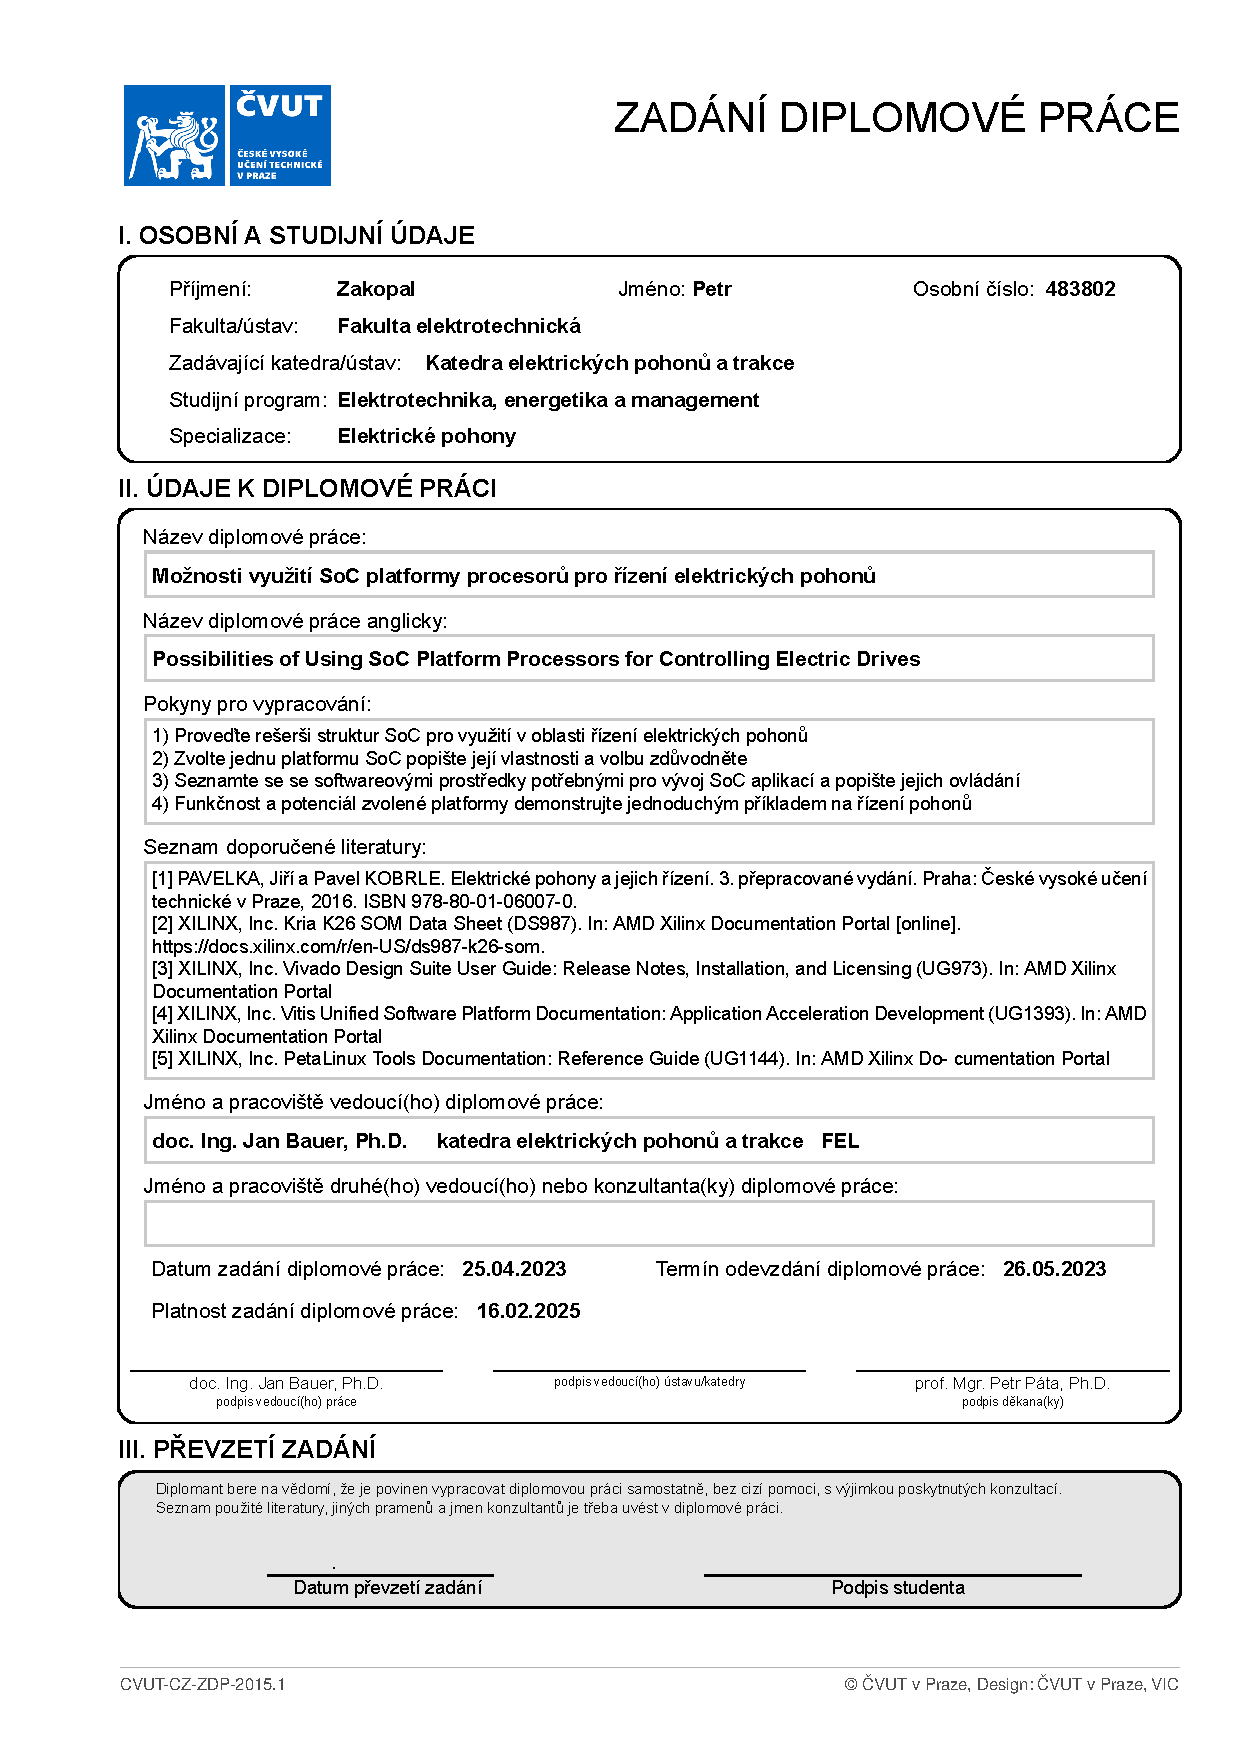
\includepdf[]{src/docs/zadani_bez_podpisu.pdf}

%\newpage
%\cleardoublepage
\null\newpage

\pagenumbering{Roman}
\setcounter{page}{5}%%3 NUTNO řešit dle zadání etc.

\noindent \textcolor{ctublue}{{\Large{\textbf{\MakeTextUppercase{Prohlášení}}}}}\\
			Prohlašuji, že jsem předloženou práci vypracoval samostatně a že jsem uvedl veškeré použité informační zdroje v~souladu s~Metodickým pokynem o~dodržování etických principů při přípravě vysokoškolských závěrečných prací.\\
		\vspace{1.5cm}
		
	

	\noindent	V~Praze dne \rule{3.5cm}{0.4pt} \hspace{6.6cm}  \rule{4cm}{0.4pt}
	
	\hspace{12.65cm}Petr Zakopal


		\vspace{14cm}
		
	\noindent	\textcolor{ctublue}{{\Large{\textbf{\MakeTextUppercase{Poděkování}}}}}\\
	Nam quis commodo justo. Mauris diam metus, mattis sed rutrum in, volutpat sit amet sem. Nam bibendum commodo porttitor. Quisque eget lectus rutrum, molestie tortor id, iaculis nunc. Sed et maximus ipsum. Vivamus vel facilisis nisl. Curabitur eu nibh nec erat mollis finibus at in sapien. Mauris viverra sapien neque, nec lacinia odio laoreet eu. Quisque consectetur eros ac orci interdum scelerisque.
		


%%ABSTRAKT%%

\newpage
%\addcontentsline{toc}{section}{3\quad Abstrakt a klíčová slova}%Added citations to TOC%
%\begin{comment}
\begin{minipage}[t]{7.37cm}
		%\raggedright
	\textcolor{ctublue}{\Large{\textbf{\MakeTextUppercase{Abstrakt}}}}\\
	Nam quis commodo justo. Mauris diam metus, mattis sed rutrum in, volutpat sit amet sem. Nam bibendum commodo porttitor. Quisque eget lectus rutrum, molestie tortor id, iaculis nunc. Sed et maximus ipsum. Vivamus vel facilisis nisl. Curabitur eu nibh nec erat mollis finibus at in sapien. Mauris viverra sapien neque, nec lacinia odio laoreet eu. Quisque consectetur eros ac orci interdum scelerisque.\\
	\textbf{Klíčová slova:} Lorem ipsum dolor sit amet, consectetur adipiscing elit. Duis aliquam finibus sagittis. Nunc venenatis, augue quis luctus dictum, elit justo pharetra leo, nec viverra purus dui at quam.
\end{minipage}%
\hfill% --- important, otherwise it wont be so nice
\begin{minipage}[t]{7.37cm}
		\textcolor{ctublue}{\Large{\textbf{\MakeTextUppercase{Abstract}}}}\\
		Nam quis commodo justo. Mauris diam metus, mattis sed rutrum in, volutpat sit amet sem. Nam bibendum commodo porttitor. Quisque eget lectus rutrum, molestie tortor id, iaculis nunc. Sed et maximus ipsum. Vivamus vel facilisis nisl. Curabitur eu nibh nec erat mollis finibus at in sapien. Mauris viverra sapien neque, nec lacinia odio laoreet eu. Quisque consectetur eros ac orci interdum scelerisque.\\
		\textbf{Keywords:} Lorem ipsum dolor sit amet, consectetur adipiscing elit. Duis aliquam finibus sagittis. Nunc venenatis, augue quis luctus dictum, elit justo pharetra leo, nec viverra purus dui at quam.
\end{minipage}
%\end{comment}
	%\textcolor{ctublue}{\Large{\textbf{\MakeTextUppercase{Abstrakt}}}}\\

	%\textcolor{ctublue}{\Large{\textbf{\MakeTextUppercase{Abstract}}}}\\

\newpage
\tableofcontents
\newpage%
\flushbottom %vyčištění stránky
\newpage
\vspace{0pt}
\listoffigures %seznam obrázků
\flushbottom %vyčištění stránky
\newpage
\listoftables
\flushbottom
\newpage


\pagenumbering{arabic} %to arabic page numbering - enabling page numbering after gobble which disabled page numbering
\pagenumbering{gobble}
\null\newpage
\null\newpage %PŘI VERZI ONLINE
\setcounter{page}{1}
\pagenumbering{arabic}
\fontspec{Times New Roman}

\section{Úvod}
V době, kdy byla od elektrických pohonů požadována spolehlivost, vysoká účinnost a nenáročné ovšem kvalitní řízení, byly k řízení využívány samotné digitální signálové procesory. Postupem času dochází ke zjištění, že výkon DSP není dostatečný a na některé aplikace, kde je vyžadováno provedení značné množství náročných výpočtů za co nejkratší čas, nejsou vhodné. Proto nastupuje éra logických programovatelných polí (FPGA), které jsou schopny tyto výpočty provést s velmi nízkými nároky na energii a za velmi krátký čas.\par
V mnoha odvětvích se již začíná využívat embedded systém s Application Spefified Hardware, který je určen pouze na využití v předem dané aplikaci. Tento hardware slouží v dané aplikaci k jedinému účelu, který vykonává a na který je optimalizován. Tím se liší od procesoru, který vykonává mnoho instrukcí a využít ho pouze jako samostatnou výpočetní jednotku je z hlediska energetické i finanční náročnosti nevýhodné. Implementace hradlových polí přináší nejen v řízení elektrických pohonů zvýšení výpočetního výkonu, ale také snižování energetické náročnosti řízení.\par
Perspektiva logických programovatelných polí a hardwaerově urychlovaných aplikací je podpořena jejich využíváním i mimo obor elektrických pohonů a trakce. Z důvodu jejich veliké propustnosti, vysokých výpočetních výkonů a nízké energetické náročnosti jsou využívány v AI, machine learningu, zpracování obrazu, těžení kryptoměn a jiných nepohonářských aplikacích.\par
Nevýhodou problematiky FPGA je jejich složitější programovatelnost z hlediska tvoření aplikace. Aplikace je tvořena určitým postupem (workflow), který kladne vysoké nároky na vzdělání a zkušenosti vývojářů. Většina FPGA je programována pomocí jazyků Verilog či VHDL, které mohou pro softwarově orientované programátory představovat značnou překážku. Proto bylo vyvinuto tvoření aplikací pomocí vyšší úrovně syntézy (HLS), kdy je možné tvořit programy ve vyšších programovacích jazycích jako je například C, C++ či Python. HLS umožnilo rapidní rozšíření a využití Embedded FPGA Accelerated Applications v mnoha aplikacích a značně vylepšilo vývojářský požitek (developer experience, DX) při tvorbě aplikací.\par
Protože může být náročné vytvořit vlastní architekturu, složenou z CPU a spolupracujícího FPGA, je vhodné při prvotním vývoji aplikace využít dostupné vývojové desky obsahující již předpřipravené propojení jednotlivých komponent. Součástí těchto vývojových desek bývá také mnoho vstupů a výstupů (I/O) pro snadnější využití při lazení a tvoření aplikace. V této práci je využívána vývojová deska Zybo od firmy Digilent. Ovšem autor v textu představuje další možnosti, které mohou být pro konkrétní aplikace a využití vhodnější.\par
Tato práce se zajímá o aplikace a možné využití FPGA při řízení elektrických pohonů. Autor v ní představuje základní principy Hardware Accelerated Applications, z jakého důvodu je tento přístup perspektivní a proč je vhodné se orientovat tímto směrem.\par
\flushbottom %vyčištění stránky
\newpage
%konec úvodu

	\section{Embedded Systems}
	Embedded systémy je název pro skupinu zařízení, obecně systémů, které je možné charakterizovat jako specifické výpočetní zařízení, resp. počítače, které jsou určeny pro podporu funkce nebo řízení nějakého většího celku, produktu nebo fyzikálního systému. Oproti tomu osobní počítač je sice výpočetní zařízení, ale nelze mluvit o embedded systému, protože je určen pro mnoho univerzálních aplikací. \cite{Sass2010}\par
	Dalším důležitým rozdílem mezi \textit{Embedded System} a obecným výpočetním zařízením je ten, že v případě embedded systému je interakce mezi systémem a uživatelem uměle omezena na základní ovládání či kontrolu funkce. Není předpokládáno, že by uživatel, jež aplikaci embedded systému využvá, výrazným způsobem zasahoval do jeho funkce. Naopak obecný výpočetní systém je uzpůsoben na podstatné zásahy uživatele. \cite{Sass2010} \cite{juan-fpgas}\par
	Do embedded systému obecně vstupují vstupní signály, které jsou následně zpracovány a poté vybrané výsledky výpočtů jsou v podobě výstupní signálů výstupním produktem systému. Tyto produkty mohou pomocí akčních členů zasahovat do řízeného systému či aplikace. Vstupní signály většinou přicházejí ze speciálních snímačů, kompatibilních s embedded systémem (senzor teploty, senzor tlaku, senzor zrychlení, gyroskop apod.). Naopak jeho výstupem signály, vedoucí na konektory, na kterých se dle požadavků objevuje např. specifická hodnota napětí. Nebo mohou na výstupních pinech být připojené LED signalizace, komunikační sběrnice některých komunikačních systémů nebo výstupní LDC displaye. Způsob, kterým jsou kódovány vstupní a výstupní signály je většinou specificky určený aplikaci daného systému. \cite{Sass2010}\par
	K obecnému výpočetnímu systému je možné připojit vstupní periferie klasických osbních počítačů – myš, klávesnice, mikrofon. Jako hlavní výstupní periferie obecného systému je monitor. Jeho komunikace s periferiemi je většinou standardizována tak, aby bylo možné periferie libovolně zaměňovat bez změny funkčnosti. \cite{Sass2010}.\par
	Na obrázku \ref{fig:embedded-system-scheme} je zobrazeno názorné blokové schéma řízení fyzikálního systému pomocí embedded systému. Tyto bloky mezi sebou komunikují pomocí digitálních signálů. Pokud tyto signály nejsou digitální, musí se před zpracováním v embedded systému zdiskretizovat.

	\begin{figure}[htbp!]
		\centering
			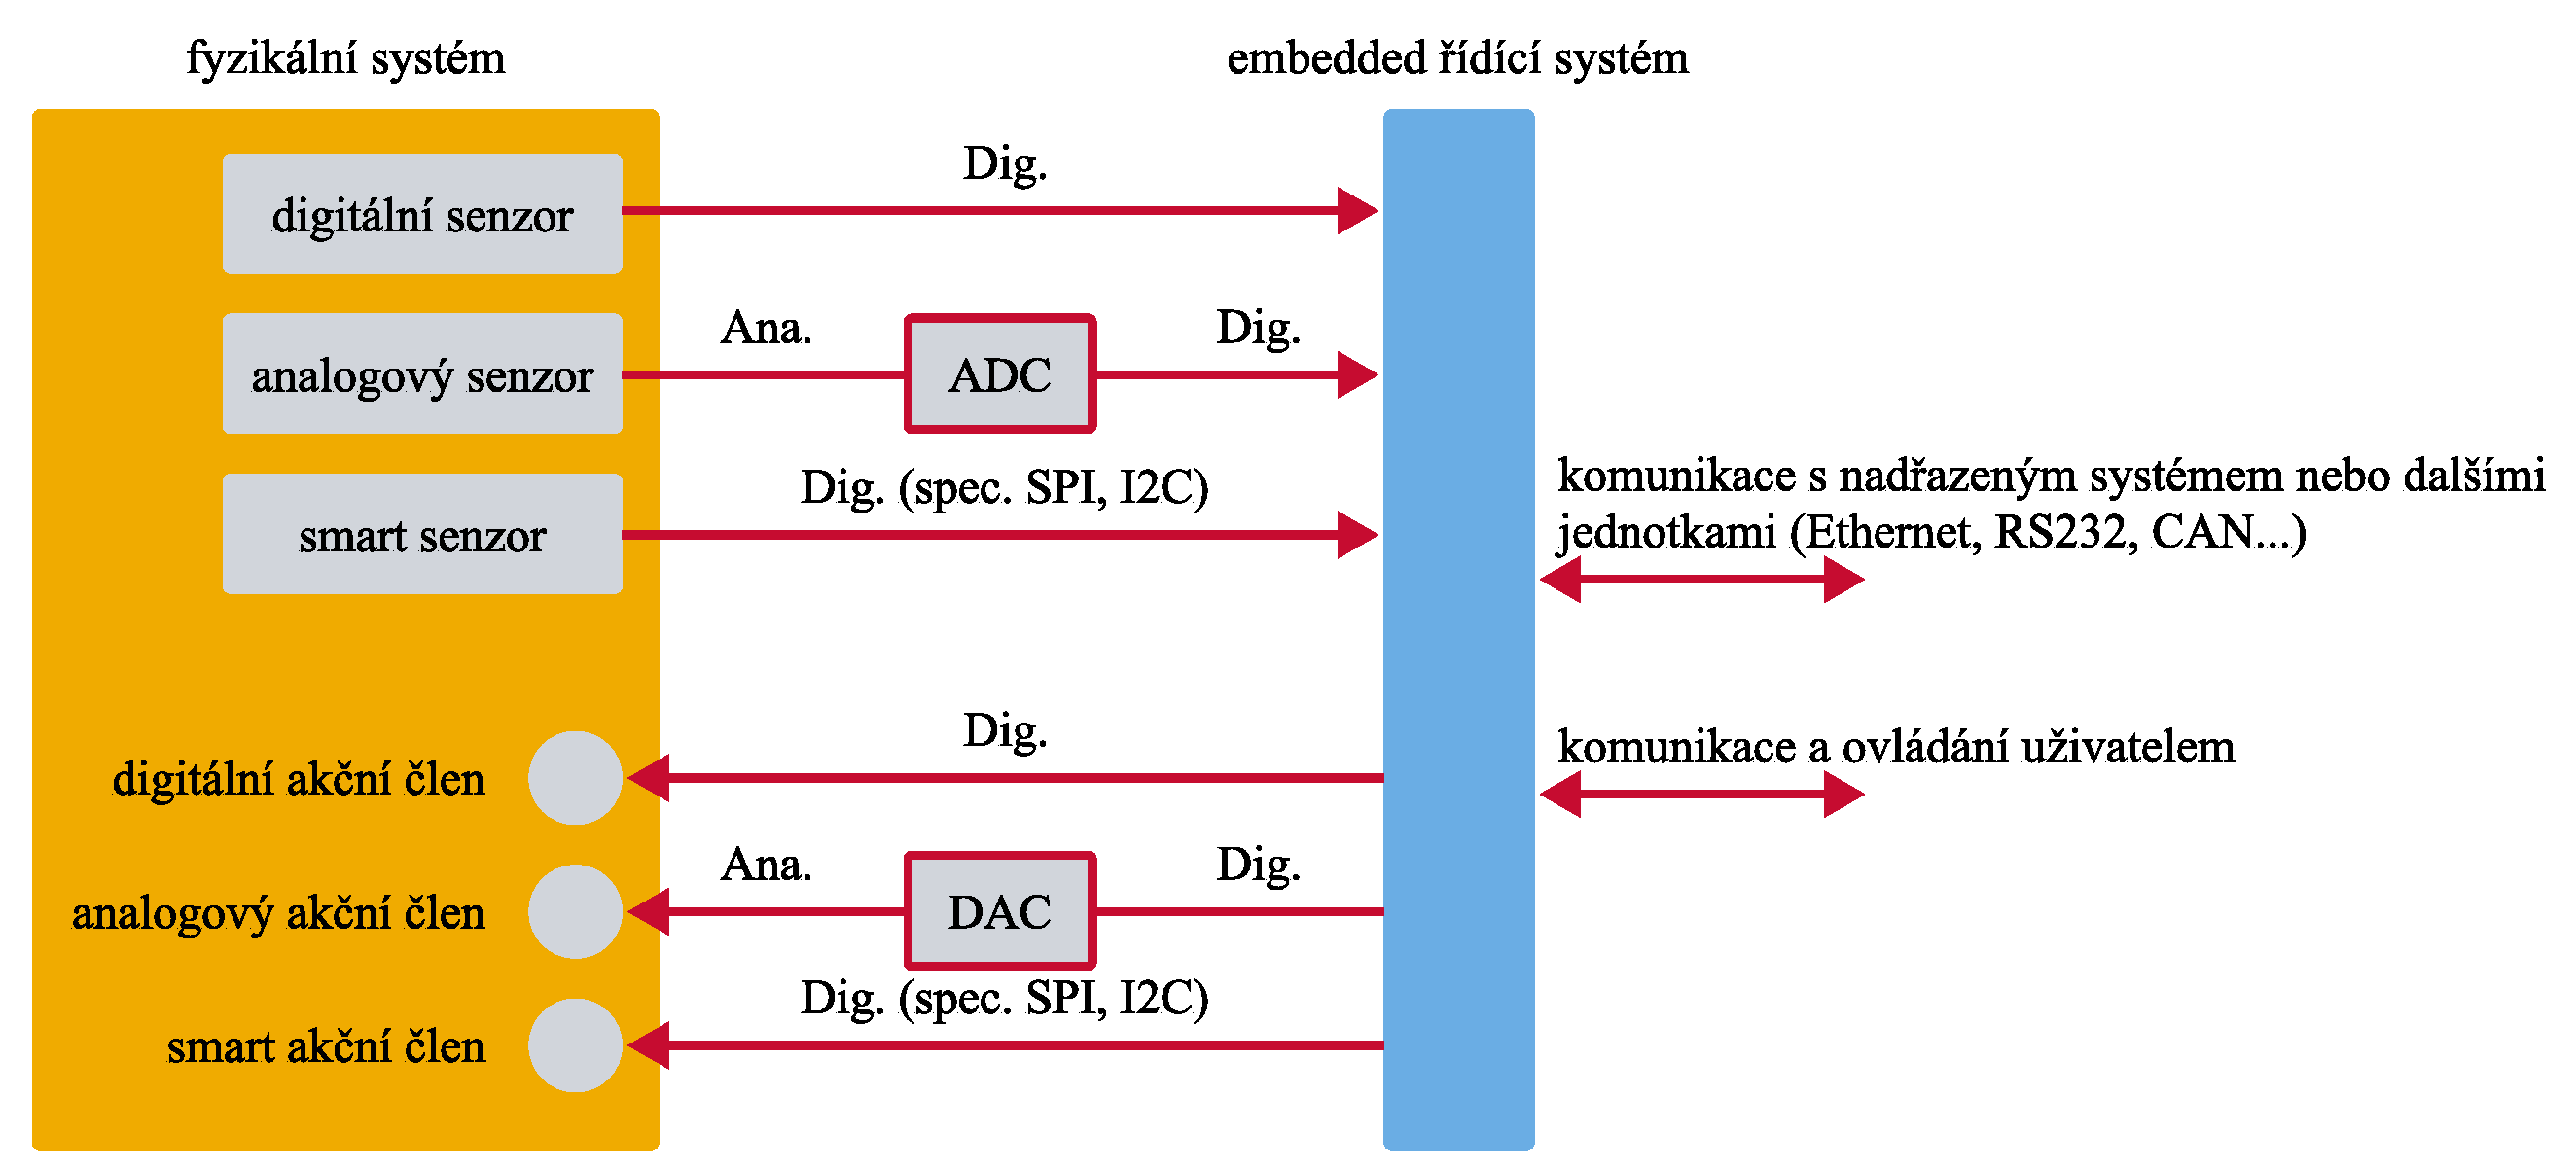
\includegraphics[width=1\textwidth]{src/pdf/embedded-system-scheme.pdf} 
			\caption{Blokové schéma Embedded systému a řízeného fyzikálního systému. (převzato a upraveno z \cite{juan-fpgas})}
			\label{fig:embedded-system-scheme}
	\end{figure}

		\fbar
		\subsection{Application Specific Integrated Circuit}
		S tématem embedded systémů se pojí pojem hardware, který je určen pro jedinou aplikaci. Tato skupina zařízení se nazývá \textit{Application Specific Integrated Circuits, popř. Hardware} (ASICs, ASHW). V této oblasti je opět využíváno přesvědčení, že pokud je architektura HW přímo specializovaná na jednu aplikaci, je vysoká pravděpodobnost, že ji bude vykonávat bezchybně, kvalitně a rychle.\par
		Tyto aplikace jsou využívaný v širokém spektru oborů jako je např. zpracování zvuku, videa, výpočtů apod. Tyto ASIC mohou také vykonávat potřebné rychlé výpočty pro matematické modely elektrických strojů, které jsou využívány např. pro HIL.\par
		Než je tento specifický obvod vytvořen, je nutné jej navrhnout, vyzkoušet a odladit. K tomu slouží logická programovatelná pole, ve kterých je možné požadovaný HW navrhnut a odladit před velko produkcí ASIC. Pokud velko produkce není z ekonomických důvodů možná, jsou FPGA využívány i v produkční oblasti, kde je HW struktura, která by byla přítomna na ASIC, vytvořena přímo na FPGA.

		\subsection{Hardware Accelerated Applications}\label{subsec:hardware-accelerated-applications}
		V mnoha aplikacích, nejen při řízení elektrických pohonů, je vyžadováno, aby výpočty nebo zpracování dat probíhalo vysokou rychlostí. Tento problém nemůže být většinou vyřešen použitím běžného procesoru (CPU), který je optimalizován na provádění obecných komplexních funkcí řízení běhu programu, komunikace či přesunu dat. V moderním světě dochází k exponenciálnímu nárůstu množství dat, které je potřeba zpracovat. Aby tyto data bylo možné v požadovaném čase zpracovat, je třeba využít specifický HW, který bude schopen požadavky rychlosti a výkonu uspokojit. Tento proces se nazývá \textit{Hardware Acceleration}. \cite{xilinx-accelerated-computing}\par
		Princip hardwaerové akcelerace spočívá v přesunu výpočetně náročných aktivit na zvláštní oddělený hardware. Celkové řízení běhu aplikace a komunikace je ovšem stále přítomno na řídícím CPU. Oddělený hardware, na kterém dochází k akceleraci výpočtů je optimalizován na vykonávanou úlohu a jeho využití přináší zefektivnění běhu celkové aplikace. \cite{xilinx-accelerated-computing}\par
		Struktura, ve které je využíváno více oddělených hardwarových procesorových a akceleračních jednotek, se často nazývá heterogenní. \cite{xilinx-accelerated-computing}\par
		Hardwaerová akcelerace poskytuje rychlejší výpočty než CPU, protože využívá značné úrovně paralelismu výpočtů. Oproti tomu klasické CPU vykonává jednotlivé instrukce sériově. I v případě, že CPU má více jader a využívá více vláken, nemůže se úrovni paralelismu při dané energetické náročnosti HW vyrovnat.\par
		Pro HW akceleraci je v mnoha oblastech využíváno několik druhů jednotek, které jsou optimální pro dané aplikace.\par
		\textbf{Graphics Processing Units} (GPUs) jsou jednotky, které převážně slouží k akceleraci zpracování a renderování grafických úloh. V době rapidního rozvoje elektroniky a SW je možné využití GPUs v mnoha odvětví umělé inteligence (AI) či kreativních odvětích. GPUs jsou využívány v aplikacích, kde není kladen veliký důraz na nízkou odezvu (latenci). \cite{xilinx-accelerated-computing}\par
		\textbf{Tensor Processing Units} (TPUs) jsou jednotky, které slouží k provádění algoritmů strojového učení (machine-learning, ML). Jejich přímé datové propojení umožňuje velmi rychlý a přímý přenost dat. Díky přímému připojení nevyžadují využití pamětí, kter= by přenos dat zpomalovali. \cite{xilinx-accelerated-computing}\par
		\textbf{Field Programmable Gate Arrays} (FPGAs) jsou jednotky, ve kterých není při výrobě pevně daná HW struktura. To umožňuje vytvoření, resp. naprogramování HW dle požadavků akcelerované aplikace. FPGAs jsou využívány i v on-line výpočtech matematických modelů elektrických strojů. Při realizaci této práce je pro akceleraci využíváno právě těchto programovatelných polí.

	\section{Programovatelné hradlové pole – FPGA}
		\subsection{Vývoj FPGA z PLD}
		Programovatelné hradlové pole jsou zařízení, jejichž historický vývoj stojí na programovatelných logických zařízení (programmable logic devices, PLD). První PLD fungovala na principu Booleových funkcí součtu násobení (sum of products). Tyto zařízení obsahovala matici více vstupových bloků AND a OR. Programování požadované probíhalo pomocí přerušování vstupů do těchto logických bloků. Později byly do PLA přidány D klopné obvody s multiplexory. Díky těmto součástím bylo možné vytvářet logické kombinační a sekvenční obvody, resp. automaty. Posledním vylepšením PLA, které stálo před zrodem FPGA, spočívalo v umístění více PLA bloků (skládajících se z AND, OR, multiplexeru a D klopného obvodu) na jeden integrovaný čip. Programovatelné spojení různých PLA bloků a výstupů umožnilo vytvořit požadovanou funkci. \cite{Sass2010}\par

		\subsection{Aktuální složení FPGA}
		Moderní FPGA se skládají z 2D matice propojených programovatelných logických bloků, bloků speciálních funkcí a propojů vytvořených pomocí CMOS technologie. Po obvodě FPGA jsou rozmístěny vstupní a výstupní piny (I/O), připojené na zvláštní logické bloky. Použité logické bloky se skládají z mnoha logických buněk, které se skládají z generátorů funkcí a paměťových elementů. \cite{Sass2010}\par
		Na obr. \ref{fig:fpga-general-design} je možné pozorovat názorné schéma základního konceptu uspořádání FPGA. Na schématu jsou vyznačeny logické bloky, jejich propojení, propojovací matice pro aktivování jednotlivých propojů a vstupů a výstupů (I/O) FPGA.\par
		I přesto, že se tato práce věnuje využití FPGA pro řízení elektrických pohonů je vhodné představit základní části FPGA a nastínit jejich funkci.

		\begin{figure}[htbp!]
			\centering
				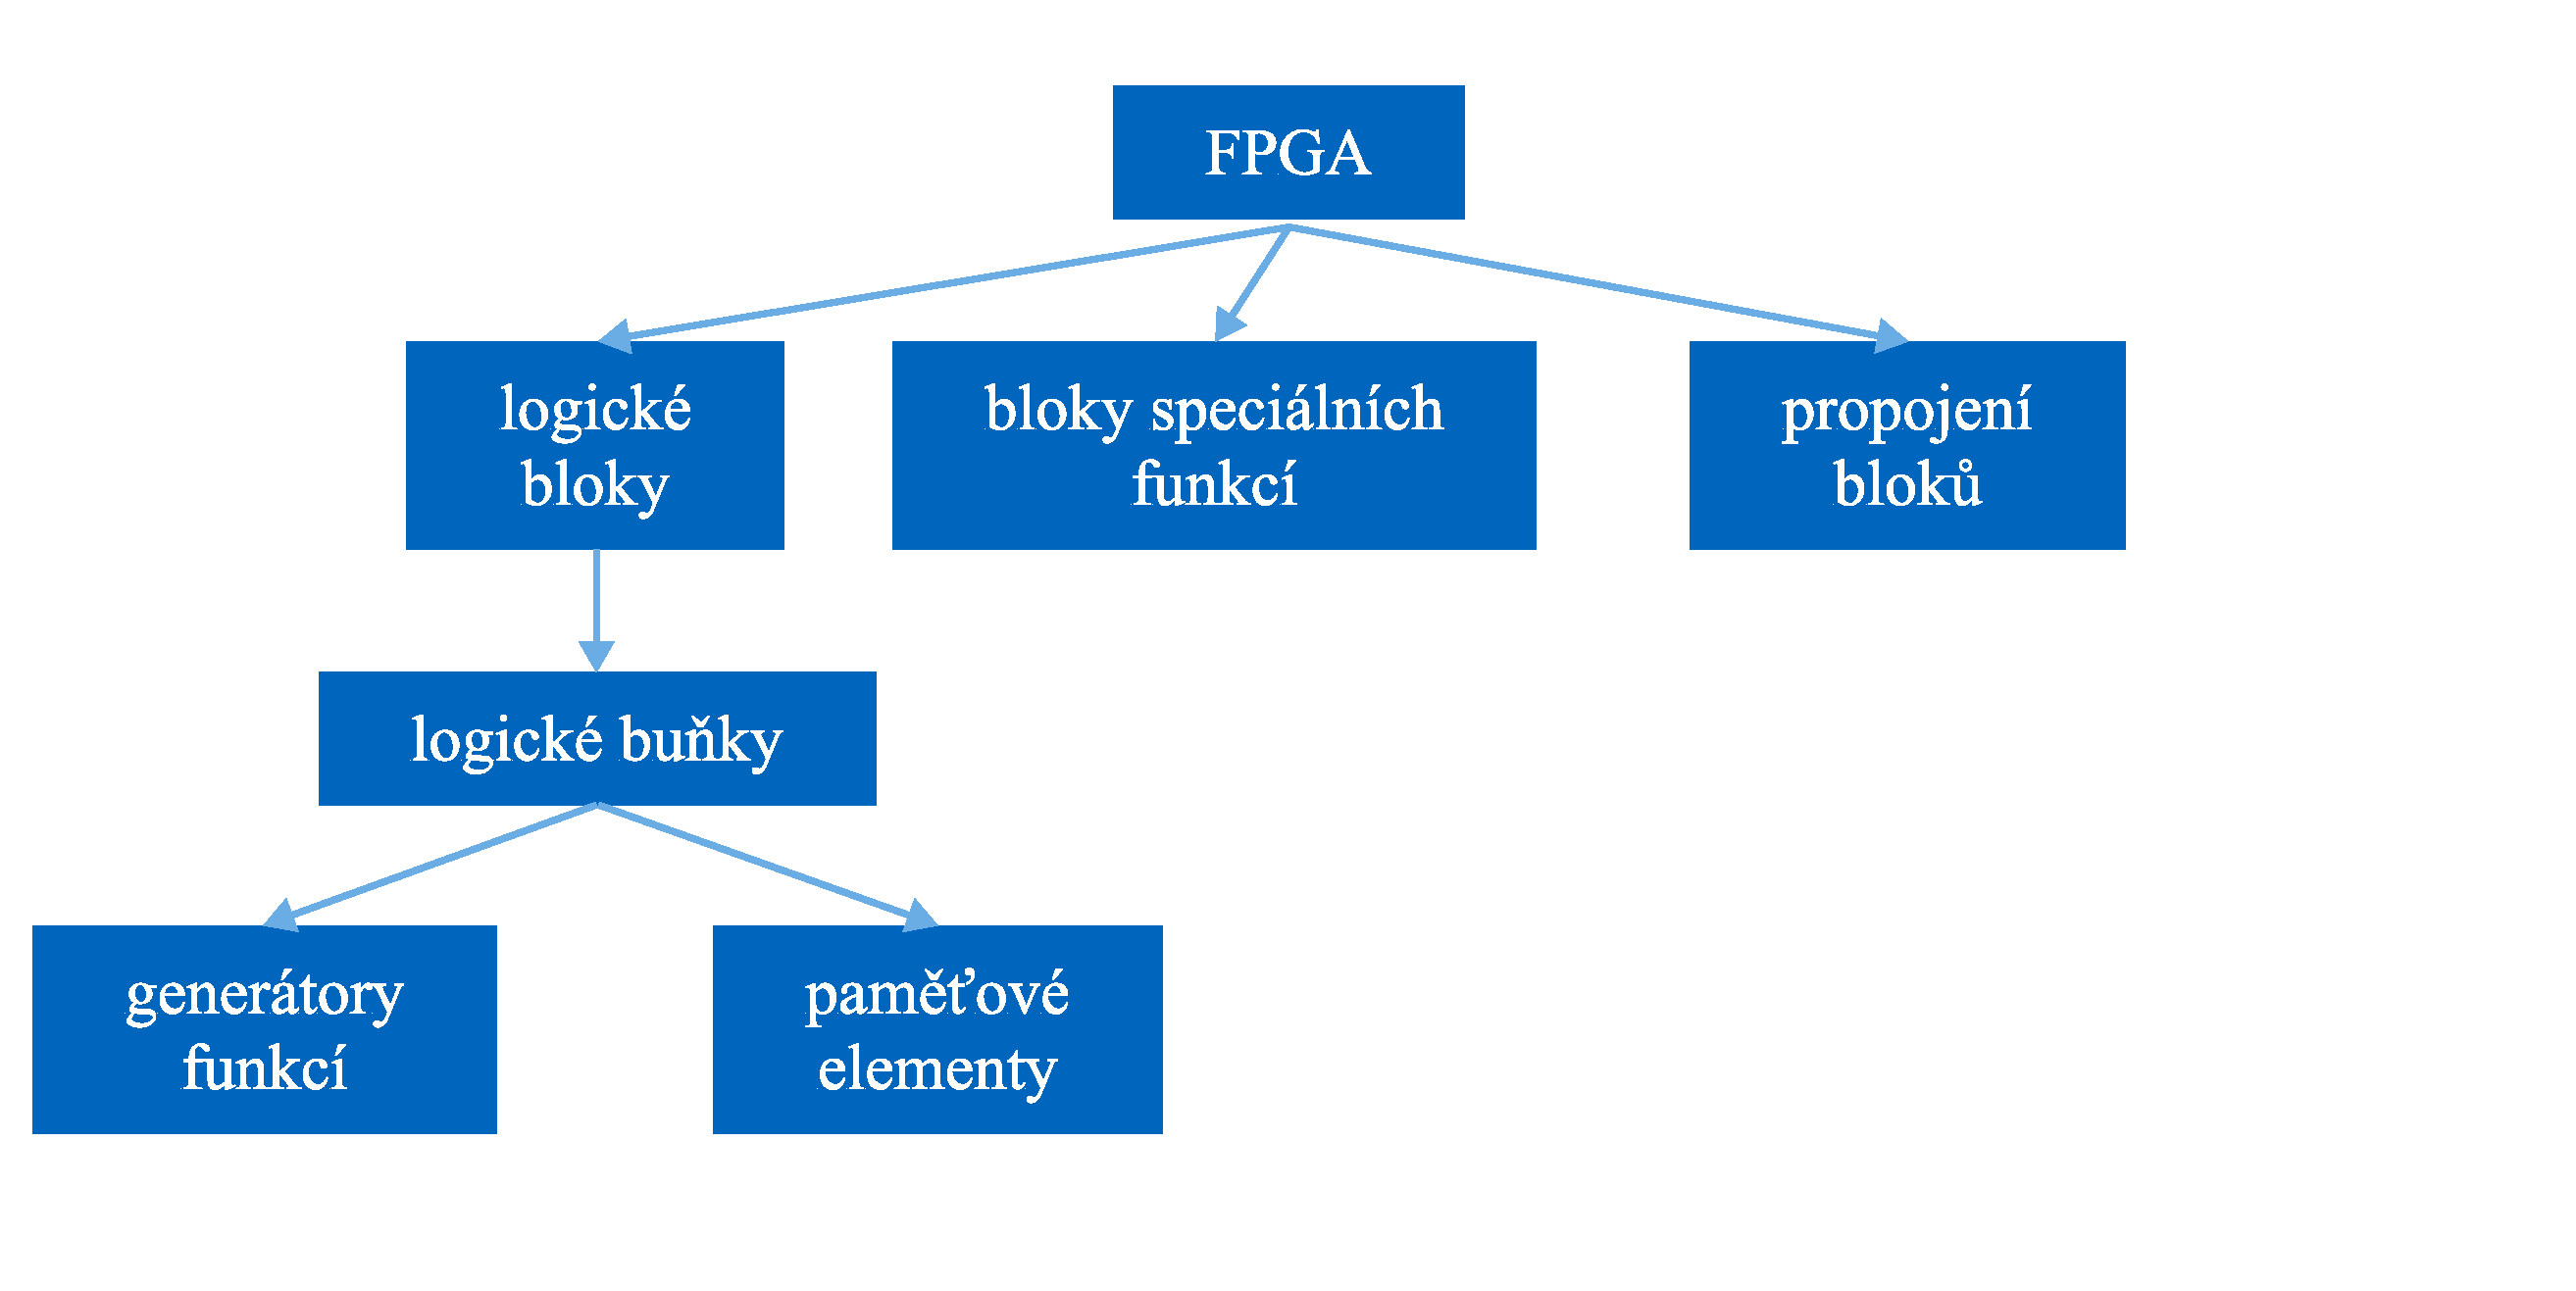
\includegraphics[width=1\textwidth]{src/pdf/fpga-skladba.pdf} 
				\caption{Blokové schéma složení moderních FPGA.}
				\label{fig:fpga-skladba}
		\end{figure}


		\begin{figure}[htbp!]
			\centering
				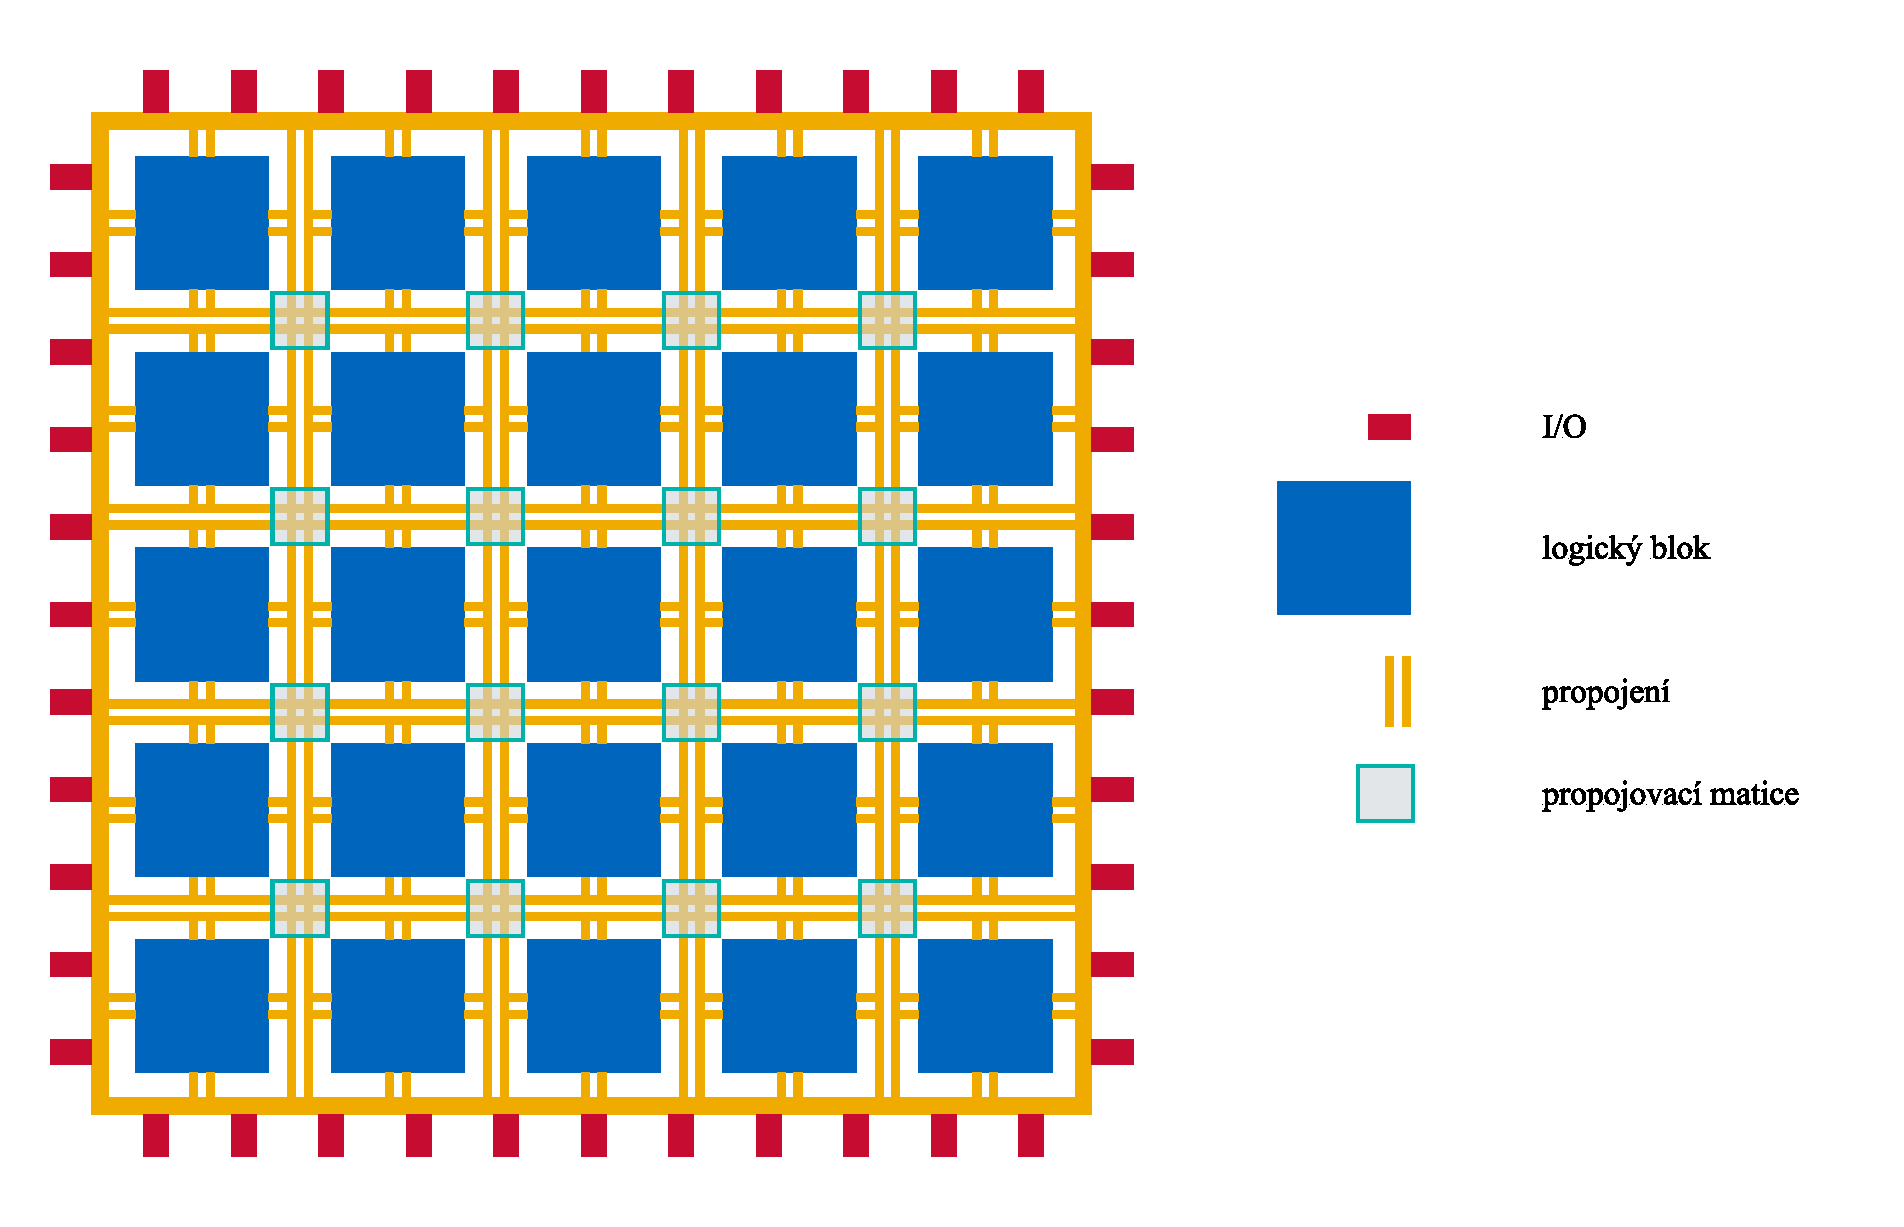
\includegraphics[width=1\textwidth]{src/pdf/fpga-general-design.pdf} 
				\caption{Základní koncept uspořádání FPGA.}
				\label{fig:fpga-general-design}
		\end{figure}

		\fbar
		\subsubsection{Generátory funkcí}\label{subsubsec:generatory-funkci}
		Oproti předchůdcům PLD, které pro generování funkcí používaly logická hradla tvořená CMOS tranzistory, využívají FPGA generátory funkcí.\par
		Logickou funkci je možné popsat pravdivostní tabulkou, která má určitý počet vstupů a odpovídající počet výstupů. Dle \cite{Sass2010} je možné si představit, že se generátor dané funkce skládá ze samostatné statické paměti (SRAM), jejíž výstupy jsou přímo přivedeny na vstup multiplexeru (MUX). Signály výběru výstupů by odpovídaly vstupním proměnným a jednotlivé vstupy do MUX výstupům funkce.\par
		Pro bližší pochopení funkce generátoru funkcí z předchozího odstavce je možné představit realizaci smyšlené logické funkce $\text{f} (x, y, z) = \bar{x}z + y$. Pravdivostní tabulka této smyšlené logické funkce je zobrazena v tab. \ref{tab:fpga-pravdivostni-tabulka-smyslene-funkce-generatoru-funkci}. Odpovídající realizace pomocí MUX a SRAM je zobrazena na obr. \ref{fig:fpga-function-generator}. Tato reprezentace se nazývá look-up table (LUT). Grafické znázornění inspirováno \cite{Sass2010}.
		

	\begin{minipage}[t]{0.45\textwidth}
		\begin{table}[H]
			\centering
			\caption{Pravdivostní tabulka ukázkové funkce, realizované v generátoru funkcí, umístěném v logickém bloku FPGA.}
		  \vspace*{0.15cm}
		
			\begin{tabular}{!{\vrule width 2pt} c | c | c | c !{\vrule width 2pt} c !{\vrule width 2pt}}
			\noalign{\hrule height 2pt}
			$i$ & $x$ &	$y$ & $z$ & f($x,y,z$)\\
			\noalign{\hrule height 2pt}
			0 & 0 & 0 & 0 & 0\\ \hline
			1 & 0 & 0 & 1 & 1\\ \hline
			2 & 0 & 1 & 0 & 1\\ \hline
			3 & 0 & 1 & 1 & 1\\ \hline
			4 & 1 & 0 & 0 & 0\\ \hline
			5 & 1 & 0 & 1 & 0\\ \hline
			6 & 1 & 1 & 0 & 1\\ \hline
			7 & 1 & 1 & 1 & 1\\\noalign{\hrule height 2pt}
			\end{tabular}
			\label{tab:fpga-pravdivostni-tabulka-smyslene-funkce-generatoru-funkci}
		\end{table}
	\end{minipage}%
	\hfill% --- important, otherwise it wont be so nice
	\begin{minipage}[t]{0.45\textwidth}
		\begin{figure}[H]
			\centering
				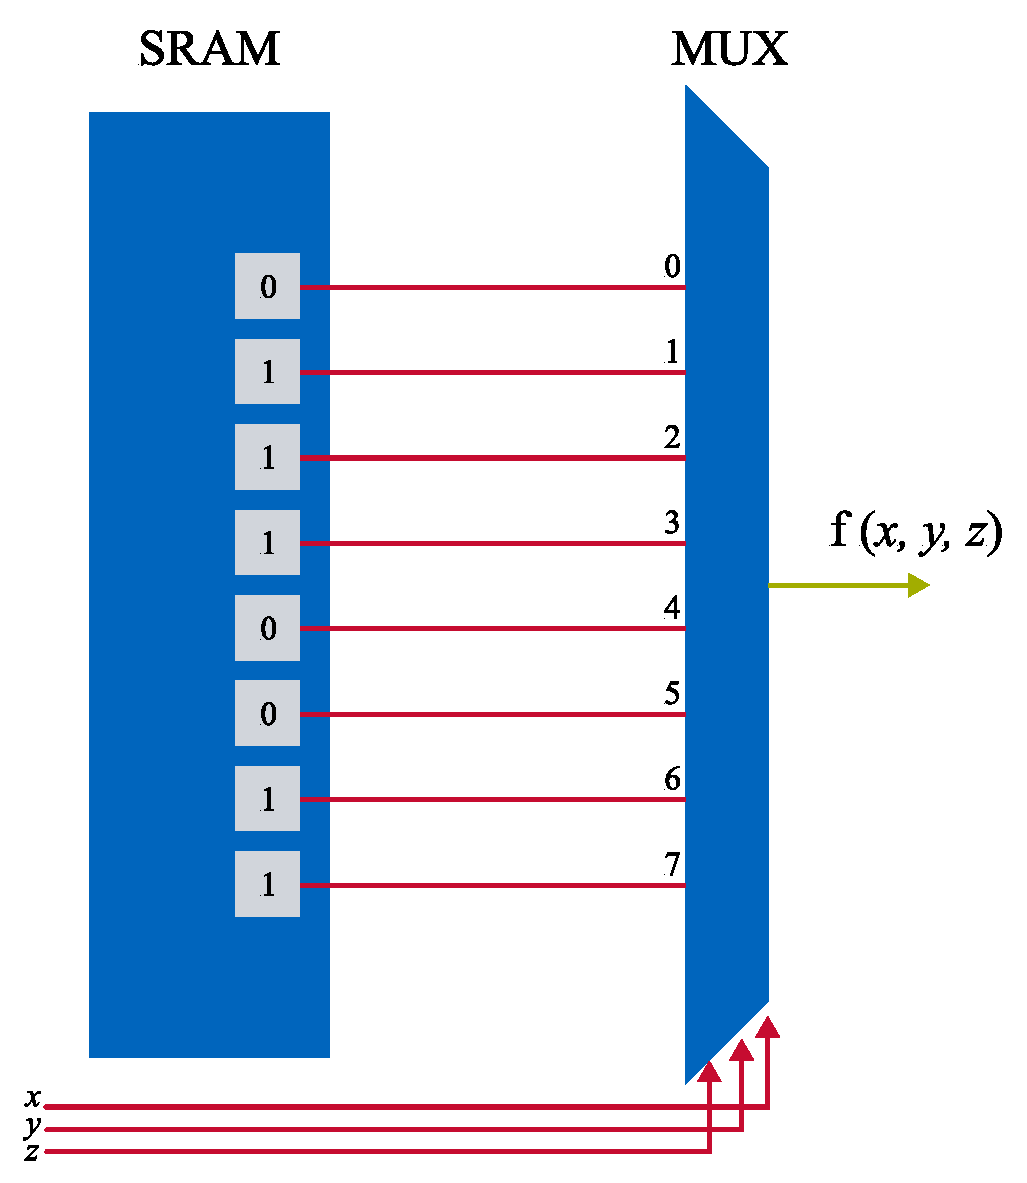
\includegraphics[width=1\textwidth]{src/pdf/fpga-function-generator.pdf} 
				\caption{Ukázka, jakým způsobem realizuje funkční generátor požadovanou funkci pomocí SRAM a MUX.}
				\label{fig:fpga-function-generator}
		\end{figure}
	\end{minipage}

	\vspace*{0.5cm}
	Výhoda této reprezentace funkcí oproti logickým hradlům je, že doba zpoždění signálu (propagation delay) pro funkci je konstantní. Respektivě je konstantní, pokud funkci je možné realizovat jednou LUT. Pro relizace obecné funkce je zapotřebí multiplexer $2^{n}$ -> 1 a SRAM s počtem buněk $2^{n}$, kde $n$ je počet vstupních proměnných dané funkce. \cite{Sass2010}

	\subsubsection{Paměťové elementy}\label{subsubsec:pametove-elementy}
		Paměťové elementy jsou v FPGA realizovány pomocí D-klopných obvodů. Tyto obvody mohou při konfiguraci FPGA být nastaveny, že budou reagovat na nástupnou nebo sestupnou hranu časovacího signálu (clock, CLK) řídícího procesoru nebo na úroveň řídícího signálu (latch).\cite{Sass2010}\par
		Protože typ latch je citlivý na úroveň signálu, může být problematické dovést požadovaný signál na vstup klopného obvodu v požadovaném čase. Velmi často jsou proto paměťové členy konfigurovány jako D-klopné obvody reagující na hranu. Pokud je používán signál CLK vyšších frekvencí, je D-klopný obvod reagující na hranu snadněji schopný reagovat v požadovaném čase. \cite{Sass2010}\par
		Často jsou na vstup paměťových elementů připojeny výstupy multiplexerů \hyperref[subsubsec:generatory-funkci]{\textit{generátorů funkcí}}. \cite{Sass2010}

		\subsubsection{Logické buňky}
			Logické buňky jsou elementy, skládájící se z \hyperref[subsubsec:generatory-funkci]{\textit{generátorů funkcí}} a \hyperref[subsubsec:generatory-funkci]{\textit{generátorů funkcí}}. Velmi často se počet logických buněk údává jako jeden ze základních parametrů FPGA, podle kterého je uživatel možný rozhodnout, zda je vhodný pro jeho aplikaci. Pomocí logické buňky nebo skupiny logických buněk je již možné vytvářet plnohodnotnou kombinační a sekvenčí logiku.\cite{Sass2010}

		\subsubsection{Logické bloky}\label{subsubsec:logicke-bloky}
			Logické bloky se skládají ze spojení několika logických buněk do jedné skupiny. Tato skupina buněk je obvykle na čipu geograficky blízko a proto dochází k minimalizaci zpoždění signálu. Velmi časté je, že jednotlivé bloky mohou mít již předkonfigurovanou funkci, jako je např. sčítačka, dělička nebo násobička. \cite{Sass2010}

		\subsubsection{Propojení bloků}
			Propojení bloků slouží ke spojení jednotlivých logických bloků a I/O. Pro spínání určených propojů jsou na čipu mezi jednotlivými propoji umístěny propojovací matice, resp. „přepínače“. Ty slouží ke spojení jinak oddělených propojů, logicých bloků a I/O. \cite{Sass2010}

		\subsubsection{I/O bloky}
				I/O bloky jsou obvykle umístěny na okraji designu FPGA. Slouží k přivedení resp. vyvedení signálů FPGA. \cite{Sass2010}

		\subsubsection{Bloky speciálních funkcí}
			Aby došlo např. ke snížení zpoždění signálu, který by bylo nutné vyvést z FPGA do externího CPU a naopak, jsou některé speciální funkce implementovány jako funkční bloky přímo do struktury FPGA. To umožňuje efektivní využití FPGA pro různorodé aplikace. \cite{Sass2010}\par
			\textbf{Block RAM} (BRAM) je blok, který slouží k uchování dat. Sice by bylo možné vytvořit paměťový blok z \hyperref[subsubsec:logicke-bloky]{\textit{Logických bloků}}, ale docházelo by k omezení využití FPGA pro jeho původní aplikace a bylo by potřeba využít mnoho bloků. BRAM mají oddělený vstup a výstup, současně s odděleným CLK. Proto je možné do BRAM zároveň data zapisovat a zároveň z něj číst. \cite{Sass2010}\par
			\textbf{DSP}, resp. digital signal processing bloky slouží ke zpracování digitálního signálu. V těchto blocích jsou implementované funkce AND, OR, NAND, NOT, násobičkya sčítačky. Mají nízkou spotřebu. DSP bloky jsou často umístěny geograficky blézko BRAM, které slouží jako „mezipaměti“ (buffer). \cite{Sass2010}\par
			\textbf{Procesor} implementovaný do struktury FPGA snižuje časové zpoždění při obsluhování FPGA. \cite{Sass2010}\par
			\textbf{Digital Clock Manager} slouží k vytvoření jiného, resp. nižšího taktovacího signálu CLK,oproti původnímu zdrojovému CLK, pro různé bloky v FPGA. \cite{Sass2010}\par
			\textbf{Multi-Gigabit Transcievers} slouží k přenosu dat takovým způsobem, aby došlo k minimalizaci vlivu ručení na přenášená data. Obecně obstarávají optimální serializaci a paralelizaci dat. \cite{Sass2010}\par
			Struktuře FPGA, která je obsauje všechny zdroje a funkcionalitu, potřebné pro kompletní realizaci aplikace, se nazývá \textit{platform FPGA}.
		\subsection{Programování}

		\subsubsection{Forma tvorby algoritmu pro FPGA}\label{subsubsec:forma-tvorby-algoritmu-pro-fpga}
		K programování, resp. konfiguraci FPGA je možné přistupovat z několika úrovní. Jednou z využívaných metod popisu požadovaného HW na FPGA je popis struktury/toku signálu obvody (structural/data flow circuits). K tomuto popisu je využíváno jazyků HDL, VHDL a Verilog (Hardware Description Language, VSIC HDL). V těchto jazycích je využíváno logických členů AND, OR, NOT nebo bloků sčítaček a násobiček. Forma popisu, jež naopak využívá vyššího programovacího jazyka než HDL je nazývána metoda popisu chování obvodů (behavioral circuits). Zatímco HDL slouží k popisu hardware s využitím nízké míry abstrakce, popis ve vyšších programovacích jazycích, které popis pomocí behavioral circuits umožňuje, je pro programátory značně příjemnější, protože využívá běžných procedurálních programovacích jazyků jako je C, C++ nebo Python. Tyto jazyky jsou následně přeloženy do HDL. Po překladu do HDL pomocí \textit{high level synthesis} (HLS) jsou provedeny kroky \textit{synthesis} (syntéza), \textit{place-and-rout} (umístění-a-pospojování) a \textit{bitgen} (generace bitstreamu). \cite{Sass2010}\par
		Při použití HLS může vzniknout situace, že bude vytvořen algoritmus, který bude takovým způsobem komplexní, že ho nebude možné syntetizovat na FPGA. Oproti tomu při použití popisu pomocí structural/data flow circuits, je prakticky vždy algoritmus syntetizovatelný. \cite{Sass2010}\par
		V praxi je k tvorbě algoritmů často využíváno vyšších programovacích jazyků a HLS, protože je tento přístup pro značný počet vývojářů SW srozumitelnější. Dalším častým přístupem v praxi je použití specializovaných SW jako je MATLAB™️ a Simulink, které při použití odpovídajících balíčků jsou schopny přeložit vytvořený algoritmus do HDL, který je poté možné dále zpracovat a použít pro konfiguraci FPGA.

		\subsubsection{Konverze HDL na konfigurační Bitstream}
			V části \hyperref[subsubsec:forma-tvorby-algoritmu-pro-fpga]{\textit{Forma tvorby algoritmu pro FPGA}} byly představeny dvě hlavní formy tvorby algoritmu pro FPGA. Tyto formy je však pro realizaci na FPGA nutné zpracovat.\par
			Všechny vyšší úrovně reprezentace algoritmů jsou převedeny na HDL. Následným krokem je \textit{syntéza} (synthesis), která slouží k převodu HDL na tzv. \textit{netlist}. Při převodu je HDL převáděna na logické členy AND, OR apod. \cite{Sass2010}\par
			Po vytvoření netlistu je nutné rozhodnout, jakým způsobem je možné a výhodné realizovat jednotlivé bloky v logických buňkách a LUT. Konečné sloučení členů závisí na rozsahu vstupů realizovatelných LUT. Proces seskupování logických členů a určování funkce LUT se nazývá mapování (MAP). Výsledkem MAP je opět netlist. Tento netlist však reprezentuje FPGA členy (LUT, klopné obvody apod.). \cite{Sass2010}\par
			Po mapování následuje proces umisťování (placement), při kterém je rozhodováno, které logické bloky budou realizovat FPGA členy, získané v kroku MAP. \cite{Sass2010}\par
			Bloky, které jsou umístěné ve struktuře FPGA je nutné spojit pomocí dostupných propojů na FPGA. Proces spojování a optimalizace propojů takovým způsobem, aby bylo minimalizováno časové zpoždění signálu, se nazývá \textit{routing}. Obvykle se proces slučuje s MAP do jedné fáze a nazývá se \textit{place-and-route}~(PAR). \cite{Sass2010} \par
			Posledním krokem je vytvoření binárního souboru, nazývaného \textit{bitstream}, který je poté vkládán do FPGA. Tento proces převede netlist z kroku PAR na nastavení SRAM v jednotlivých logických buňkách FPGA tak, aby byl vytvořen požadovaný design v FPGA. Proces také převede konfiguraci propojů a propojovacích matic do SRAM, ovládající příslušné propoje a matice. \cite{Sass2010}\par
			Soubor \textit{bitstream} je poté možný pomocí daného nástroje „nahrát nakonfigurovat jím FPGA“.

			
			\begin{figure}[htbp!]
				\centering
					
\includegraphics[width=1\textwidth]{src/pdf/fpga-hls-to-bitstream-flow-chart.pdf} 
					\caption{Blokové schéma převodu aplikace, naprogramované v procedurálním jazyce, na bitstream, který je vhodný pro konfiguraci FPGA.}
					\label{fig:fpga-hls-to-bitstream-flow-chart}
			\end{figure}

		\fbar
		\subsection{Spotřeba}
			FPGA je využívano pro akceleraci aplikací také pro svou nízkou spotřebu energie. Oproti ASICs však FPGA má stále značnější spotřebu, proto je podnikán výzkum, který má za cíl jejich energetickou náročnost snížit ale zachovat jejich výkon a spolehlivost.\par
			% Existuje mnoho článků na téma energy/power efficiency of fpgas ale v žádném není popsáno, proč je jeho spotřeba nižší, než v CPU
			Nižší potřebný výkon pro realizaci nepohonářské aplikace podporuje výzkum a článek \cite{rovere-sphery-vs-shapes}, ve kterém autoři představují svoji práci, v níž realizovali HW hru. Ve hře je hlavním úkolem aplikace výpočet stínů a odrazů materiálů. Způsob vykrlesení, který je v aplikaci použit je nazýván \textit{ray tracing}. Ray tracing je označován jako výpočetně náročný způsob, který není vhodný pro on-line aplikace ale pro vykreslování nepohyblivých obrazů, které není nutné zobrazovat v reálném čase. \cite{wikipedia-ray-tracing}\par
			% píšou jednoho jádra, ale to je divný, spíše prostě spotřeba %
			Autoři v textu popisují, že v případě využití FPGA pro výpočty v reálném čase byla jeho spotřeba 660 mW. Hru autoři vyzkoušeli spustit také na CPU platformě skládající se z Ryzen™️ 4900H 8-core/16 threads 64-bit CPU @ up to 4,4 GHz clock. V případš testování na CPU byla indikována spotřeba 33 W. Tudíž při použití FPGA spotřeba klesla přibližně 50x. \cite{rovere-sphery-vs-shapes}.\par
			I přes nízkou spotřebu energie v FPGA jsou prováděny výzkumy, jak minimalizovat disipaci elektrické energie v podobě tepla a přiblížit se tak energetické náročnosti ASICs.\par
			Disipace energie v FPGA je rozdělena na statickou a dynamickou.\par
			Statická disipace je způsobena zbytkovým proudem tranzistorů ve vypnutém stavu mezi drain a source elektrodou, mezi gate a drain a jevem nazvaným gate direct-tunneling. \cite{grover-reduction-of-power-consumption}\par
			Dynamická disipace je způsobena spínacími a vypínacími ztráty použitých tranzistorů (obvykle CMOS) a je závislá na použitém napětí, frekvenci a kapacitě přechodů, kterou je třeba nabít a vybít při spínání a vypínání tranzistorů. \cite{grover-reduction-of-power-consumption}
			\subsection{Výpočetní výkon a propustnost}
			\subsection{Využití}
			Programovatelná logická hradlová pole se pro svoji nízkou spotřebu, vysoký výpočetní výkon a klesající cenu elektroniky začínají využívat mnohem častěji v mnoha odvětví, ve kterých bylo doposavaď využíváno CPU a GPU. Aplikace FPGA je možné v rámci této práce rozdělit na nepohonářské a pohonářské.

			\subsubsection{Aplikace v nepohonářských odvětví}
				Díky univerzalitě FPGAs je možné je využít v mnoha aplikacích různých odvětví. Stále se zvyšující požadavky na výpočetní výkon urychlují nasazování FPGAs do provozů, kde jsou v současné době instalovány CPU nebo GPU.\par
				Poptávka po dostupnosti FPGA způsobila vznik Cloud služeb, které nabízí FPGA výkon on-demand. Jedním z velkých poskytovatelů je Amazon Web Services (AWS), který nabízí FPGA akceleraci v Cloudu. Tuto službu ocení především aplikace, které nejsou vázány na reálný hardware ale potřebují pouze dostupný výpočetní výkon, který mohou v průběhu tvorby, debuggingu či realizace aplikace měnit bez nutnosti pořizování výkonných a někdy drahých FPGA desek. Více o \textit{Amazon EC2 F1 Instances} služby virtuálních FPGA je dostupné na \cite{amazon-ec2-f1}.\par
				Existuje mnoho výpočetně náročných aplikací jako jsou např. výpočty finančních modelů pro ekonomiku, výpočty pro bioinformatiku, seismické modelování při hledání vzácných surovin apod. Více informací o těchto výpočetně náročných aplikacích je možné získat v \cite{wim-high-performance-computing-using-fpgas}.\par
				Na akceleraci zpracování audiovizuálních děl je převážně určeno GPU. Ovšem pro aplikace, v nichž je vyžadováno zpracování obrazu v reálném čase s minimální spotřebou energie a nízkou hmotností aplikace, je často využíváno FPGA. Aplikace využití FPGA pro vozidla, která analyzují okolní prostor jsou popsány v \cite{andina-advanced-features-and-industrial-applications-of-fpga}. Tyto aplikace nesou souhrnný název „inteligennt spaces applications“. Obvykle je pro analýzu okolního prostoru využíváno více kamer, z nichž každá obsahuje vlastní výpočetní jádro (FPGA). Díky tomu výpočetně náročné aplikace, jako např. analýza hloubky obrazu pro rozpoznání objektů, probíhá v FPGA a ostatní nenáročné výpočty a řízení v SW. \cite{andina-advanced-features-and-industrial-applications-of-fpga}\par
				Protože momentálním trendem je snižování energetické náročnosti a zvyšování výpočetního výkonu dochází neustále k vývoji nových aplikací, které využívají FPGA pro akceleraci výpočetně náročných kroků, proto není možné všechny v tomto textu obsáhnout.


			\subsubsection{Aplikace v elektrických pohonech}
			% HIL
			% Control
			% Control and Extended Kaufmann Filter
			V některých případech je elektrický pohon rozměrná a finančně náročná sestava, proto zkoumání určitých kritických stavů těchto soustav by mohlo být ekonomicky i technicky nevýhodné. V tomto případě je vhodné vytvořit přesný matematický model jednotlivých analyzovaných součástí a nezbytné náročné výpočty akcelerovat pomocí FPGA. Na základě odezvy modelu je poté možné analyzovat stavy, které by v případě analýze na reálném stroji mohly způsobit jeho destrukci či částečnou ztrátu funkčnosti. Proto se v průmyslu využívá Hardware-in-the-loop simulation (HILS), kdy je vytvořen požadovaný matematický model, který poskytuje elektrické signály do testovaného systému a na základě jeho reakce je možné vyhodnotit díky matematickému modelu jakým způsobem by se choval reálný modelovaný systém. \cite{andina-advanced-features-and-industrial-applications-of-fpga}, \cite{mathworks-discovery-hil-simulation}\par
			Kromě HIL simulace je možné FPGA využít také pro řízení elektrických pohonů. Možnosti realizace řízení AC elektrických strojů pomocí FPGA a analogově digitálních převodníků (ADC) jsou prezentovány v \cite{naouar-fpga-based-current-controllers-for-ac-machine-drives}. V dokumentu jsou popisovány tři realizace řízení, resp. regulace pohonu. Nejprve byla regulace realizována pomocí hystérézních on-off regulátorů, následně byly použity PI regulátory. Pomocí nich byl pohon regulován na základně měření a změny vektoru statorového proudu, resp. jeho složek $\alpha \beta$ po aplikování Clarkové transformace. Jako poslení prezentovaný způsob autoři realizovali model ovládání synchronního motoru na základě prediktivních regulátorů. \cite{naouar-fpga-based-current-controllers-for-ac-machine-drives}\par Všechny prezentované způsoby regulace v \cite{naouar-fpga-based-current-controllers-for-ac-machine-drives} byly před syntézou realizovány v prostředí MATLAB™️ a Simulink. Tento způsob tvorby modelů a algoritmů je v praxi upřednostňován, protože umožňuje i expertům na řízení a regulaci pracovat na dané problematice bez znalostí mikroelektroniky, programování v HDL a způsobu fungování FPGA. Oproti tomu je třeba zvážit, jaké jsou požadavky na rychlost, výkonnost a optimalizované řízení aplikace a zdali použití předpřipravených knihoven a zjednodušených nástrojů nebude mít příliš značný vliv na rychlost výpočtu a tudíž zpracování dat a řízení v reálném čase. \cite{naouar-fpga-based-current-controllers-for-ac-machine-drives}
			
	\section{Vývojová deska Digilent Zybo}
			Vývoj akcelerovaných aplikacích je možné realizovat na realativně velikém množství dostupného HW. V některých případech je design vývojových desek dokonce výrobcem uveřejňován a tudíž v případě dostatečných znalostí je dokonce možné si sestavit vlastní HW s dostupných komponent takovým způsobem, aby vyhovoval požadované embedded aplikaci. Výhodné ovšem je využít již připravená řešení vývojových desek, které zjednodušují prvotní tvorbu aplikace.\par
			V této práci je realizován vývoj aplikace na vývojové desce \textit{Digilent ZYBO Zynq-7000 ARM/FPGA SoC Trainer Board} od firmy Digilent. \cite{digilent-zybo-7000-docs} Jedná se o model vývojové desky, který byl nahrazen novějšími variantami s označením \textit{ZYBO Z7-10} a \textit{ZYBO Z7-20}, které jsou stále v aktivním prodeji. Hlavním rozdílem představených desek je verze Zynq čipu, který v moderních deskách disponuje ARM procesorem s vyšší taktovací frekvencí a s modernějším FPGA s vyšším počtem LUT, klopných obvodů a s rozsáhlejší pamětí RAM apod. Bližší porovnání specifikací těchto desek je dostupné na \cite{digilent-zybo-compare}.\par
			V další části textu jsou představeny významné komponenty vývojové desky \textit{Digilent ZYBO Zynq-7000 ARM/FPGA SoC Trainer Board}.

			\begin{figure}[htbp!]
				\centering
					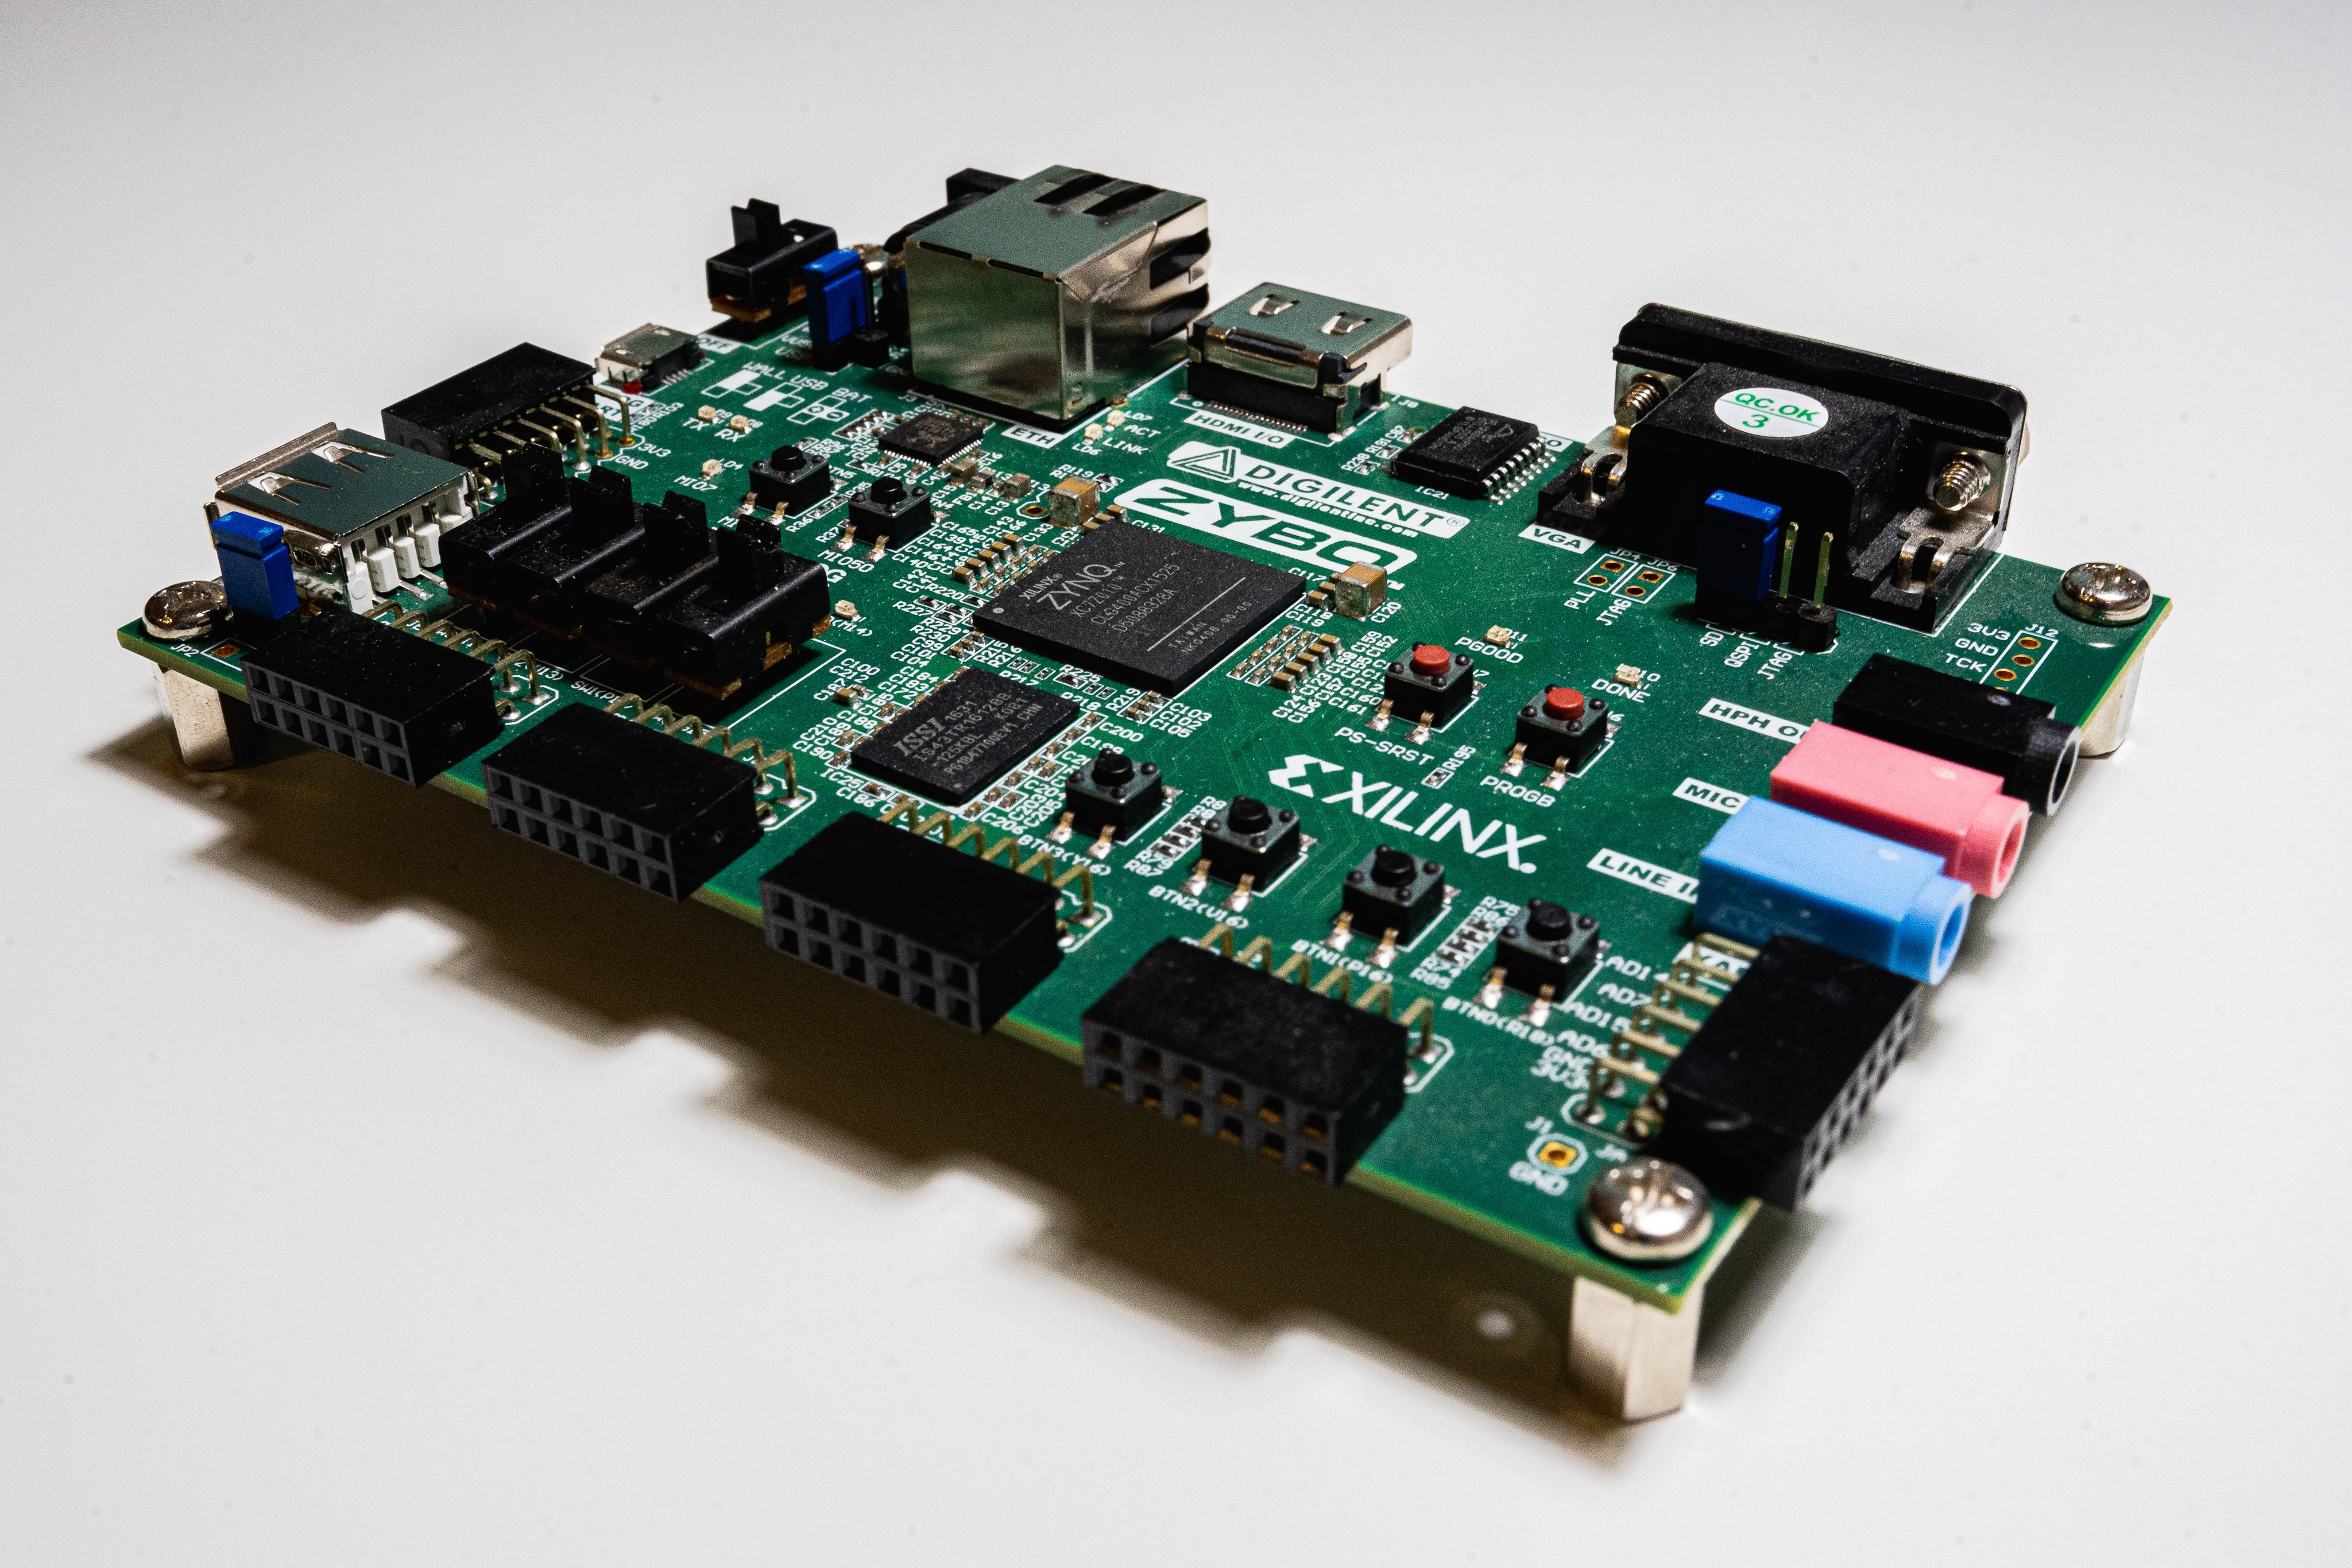
\includegraphics[width=0.85\textwidth]{src/jpg/digilent-zybo-foto-2.jpg} 
					\caption{Vývojová deska Digilent ZYBO Zynq-7000 ARM/FPGA SoC Trainer Board.}
					\label{fig:digilent-zybo-foto-2}
			\end{figure}

		\subsection{Základní přehled}
		\subsubsection{CPU a FPGA čip}
			Hlavní částí vývojové desky je čip, obsahující FPGA a CPU jednotky zakomponované v jedné polovodičové struktuře. Jak již bylo zmíněno v části \hyperref[subsec:hardware-accelerated-applications]{\textit{Hardware Accelerated Applications}}, tato struktura se nazývá heterogenní.\par
			Deska obsahuje čip Xilinx Zynq-7000 (typ XC72010), který umožňuje pro vývoj aplikací použít SDK od firmy Xilinx. V tomto čipu je integrován dvou jádrový procesor ARM Cortex-9, který slouží jako host akcelerovaných aplikací na Xilinx FPGA sedmé série. Detailní schéma blokové architektury SoC s označním sběrnic a komunikace jednotlivých částí čipu je zobrazené na obr. \ref{fig:zynq-block-diagram-detailed}.\par
			Z naznačené architektury je možné vyvodit, že se SoC skládá ze dvou hlavních částí, které je možné dále rozdělit na jednotlivé bloky:
			\begin{itemize}
				\item Processing System (PS),
				\begin{itemize}
					\item Application processor unit (APU),
					\item Memory interfaces,
					\item I/O peripherals (IOP),
					\item Interconnect,
				\end{itemize}
				\item Programmable Logic (PL).
			\end{itemize}
			\vspace*{0.25cm}
			\noindent\textbf{Blok PS}\\
			Blok PS se skládá z dílčích bloků, které neslouží k akceleraci aplikací, ale k podpoře běhu hostitelského programu. Blok PS reprezentuje prakticky celou architekturu čipu vyjma části věnované PL.\par\vspace*{0.25cm}
			\noindent\textbf{Blok APU}\\
			Blok APU obsahuje CPU Cortex-A9 a další podpůrné bloky jako např. přímý přístup do paměti (DMA controller), Genral interrupt controller (GIC) pro maskování a ovládání přerušení, watchdog a další podpůrné bloky.\par\vspace*{0.25cm}
			\noindent\textbf{Blok Memory interfaces}\\
			Memory interfaces slouží k přístupu APU a PL k pamětím typu DDR3, DDR3L, DDR2 a LPDDR-2. Je možné také vybrat, zda šířka sběrnice bude 16 nebo 32 bitů. K dispozici jsou zakoponované kotroléry přenosu dat pro optimalizaci rychlosti, Static Memory Controller nebo Quad-SPI Controller.\par\vspace*{0.25cm}
			\noindent\textbf{Blok IOP}\\
			IOP se skládá ze standardizovaných rozhraní vhodných pro průmyslovou komunikaci. Obsahuje nař. GPIO, Gigabit Ethernet, dva bloky USB Controller, dva bloky SD/SDIO Controller pro bootování SD karty, dva bloky SPI Controller, dva bloky CAN Controller, dva bloky UART Controller a dva bloky I2C Controller.\par\vspace*{0.25cm}
			\noindent\textbf{Blok Interconnect}\\
			Blok Interconnect, resp. na obr. \ref{fig:zynq-block-diagram-detailed} označený Central Interconnect slouží k propojení jednotlivých bloků SoC dle požadované technologie a rychlosti.\par\vspace*{0.25cm}
			\noindent\textbf{Blok PL}\\
			Blok PL reprezentuje logické programovtelné pole (FPGA), v němž jsou zakomponovány další podpůrné bloky jako např. blok zpracování digitálních signálů, řízení taktovacích hodin, analogově digitální převodník (ADC) apod.\par\vspace*{0.35cm}
			\noindent Veškeré technické specifikace, složení a parametry jmenovaných bloků a jsou uvedeny v \cite{xilinx-zynq-7000-technical-reference-manual}.
			% \begin{figure}[htbp!]
			% 	\centering
			% 		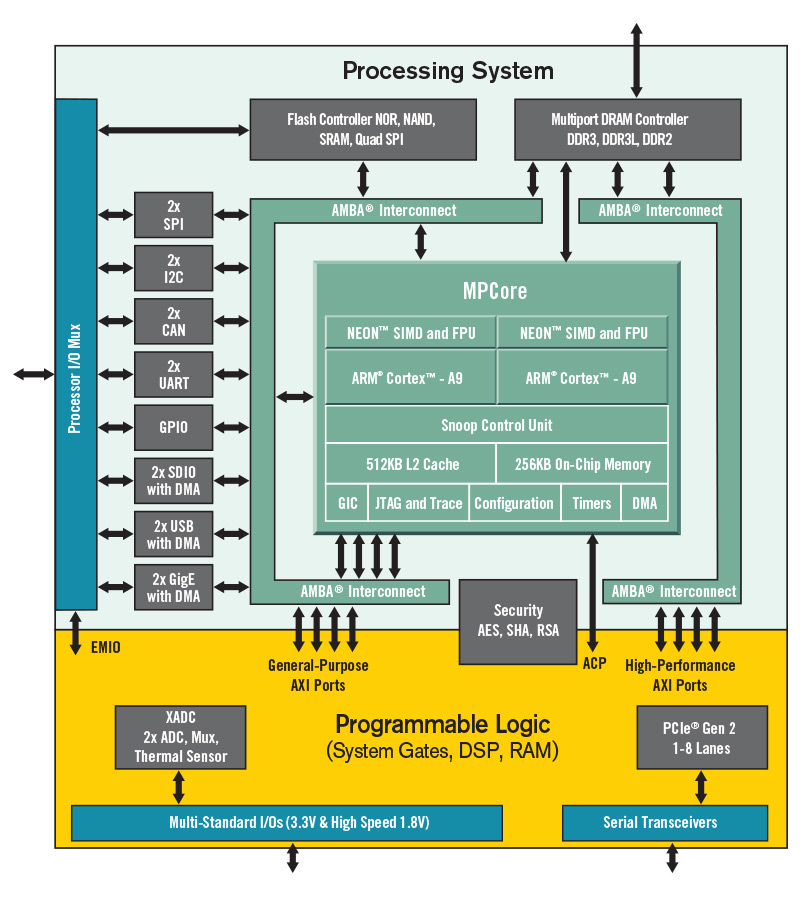
\includegraphics[width=0.75\textwidth]{src/png/zynq-mp-core-dual.png} 
			% 		\caption{Blokové schéma čipu Zynq-7000, umístěného na vývojové desce \textit{Digilent ZYBO Zynq-7000 ARM/FPGA SoC Trainer Board}. (převzato z \cite{xilinx-zynq-7000-socs-with-hardware-and-software-programmability})}
			% 		\label{fig:zynq-mp-core-dual}
			% \end{figure}

			\begin{figure}[htbp!]
				\centering
					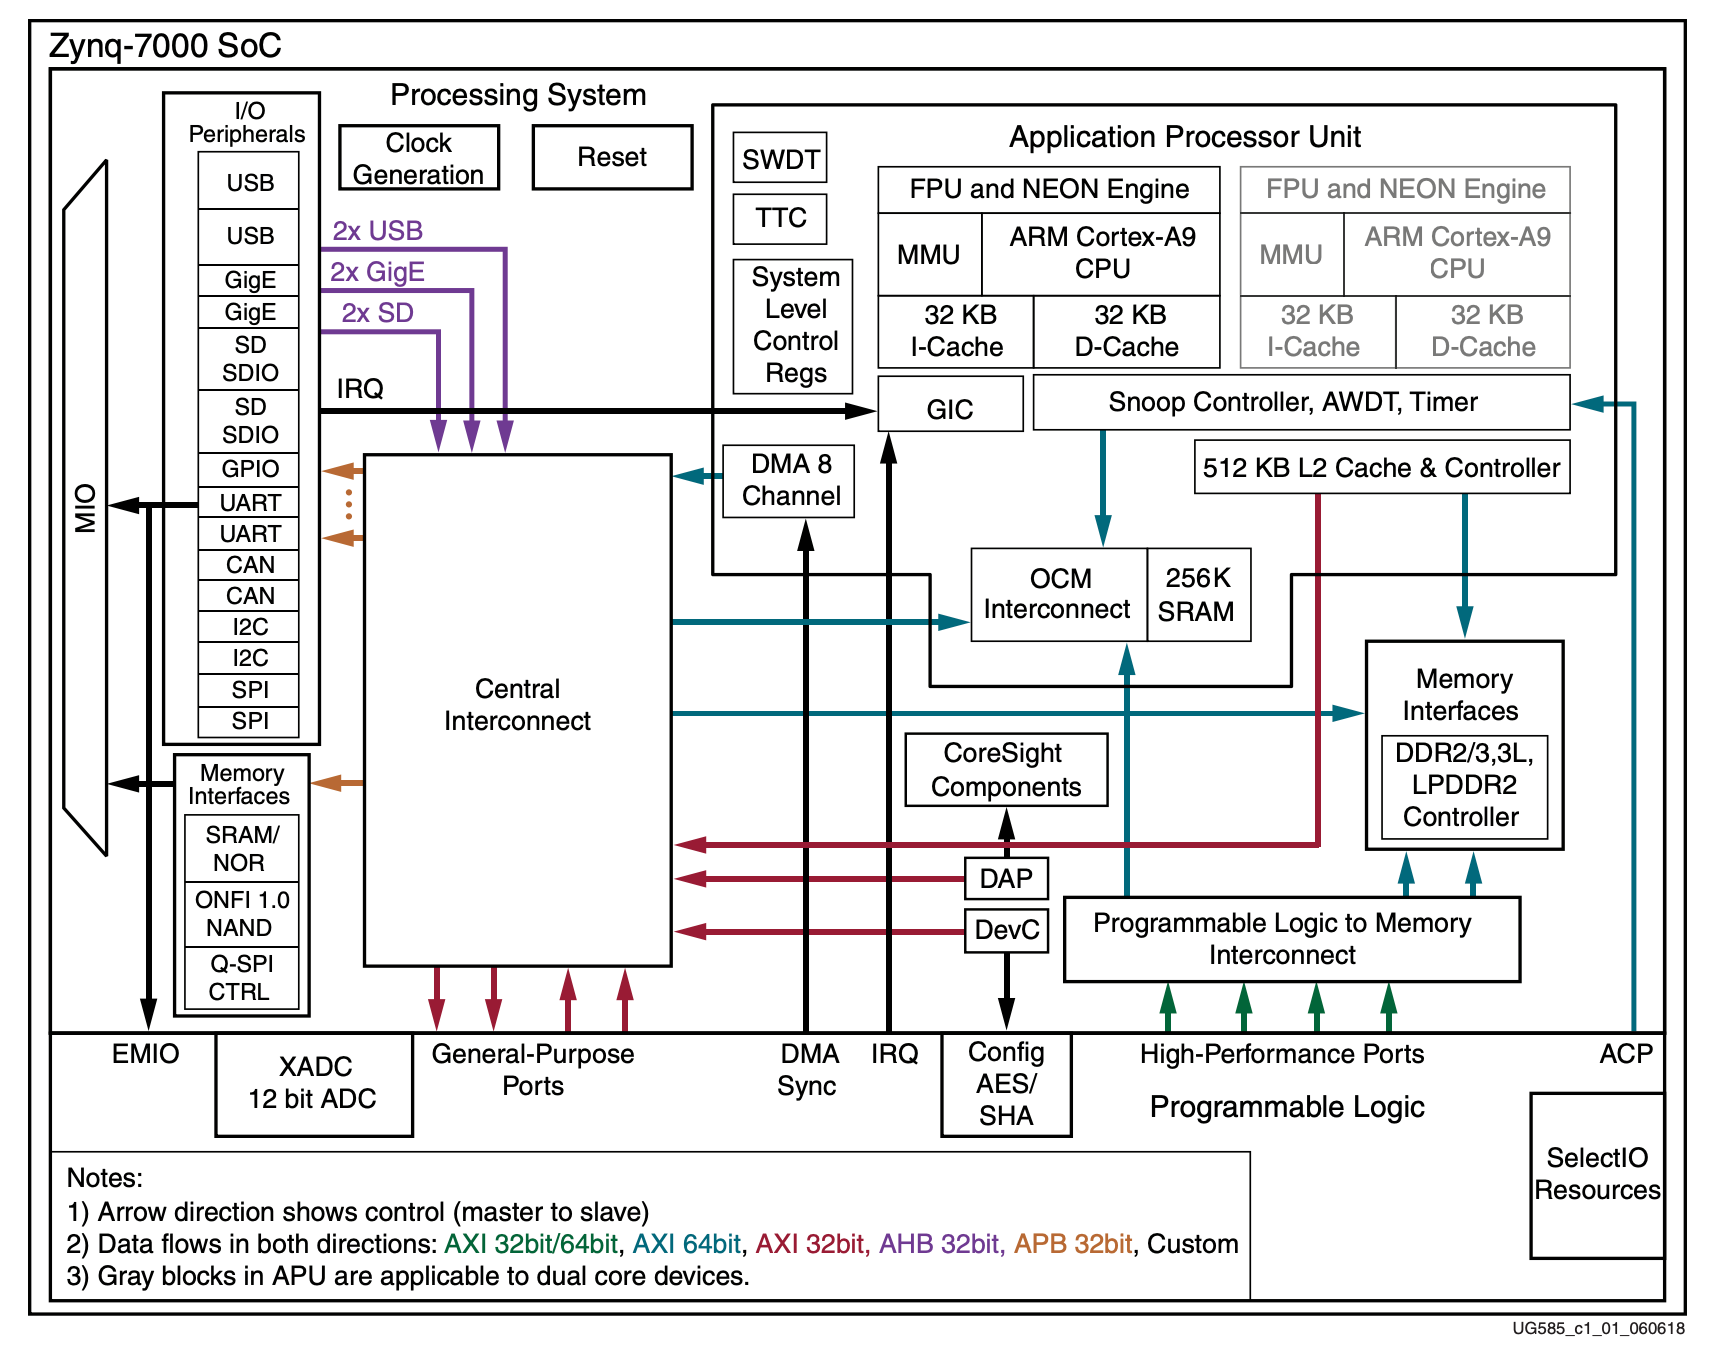
\includegraphics[width=0.90\textwidth]{src/png/zynq-block-diagram-detailed.png} 
					\caption{Detailní schéma čipu Zynq-7000, umístěného na vývojové desce \textit{Digilent ZYBO Zynq-7000 ARM/FPGA SoC Trainer Board}. (převzato z \cite{xilinx-zynq-7000-technical-reference-manual})}
					\label{fig:zynq-block-diagram-detailed}
			\end{figure}
			\fbar
			\subsubsection{Uspořádání vývojové desky Zybo Zynq-7000}
				Na obr. \ref{fig:digilent-zybo-foto-1-oznacene} je zobrazen horní pohled na vývojovou desku, na které jsou vyznačeny významné části, kterým je vhodné věnovat při práci s deskou pozornost. Číselné označení koresponduje s označením a vysvětlivkou v tabulce \ref{tab:digilent-zybo-zynq-7000-description}. Na spodní části desky se nachází menší počet součástek, které by byly významné pro ovládání a práci s deskou. Nicméně pro doplnění je spodní strana desky zobrazena na obr. \ref{fig:digilent-zybo-foto-3}.

				\begin{figure}[H]
					\centering
						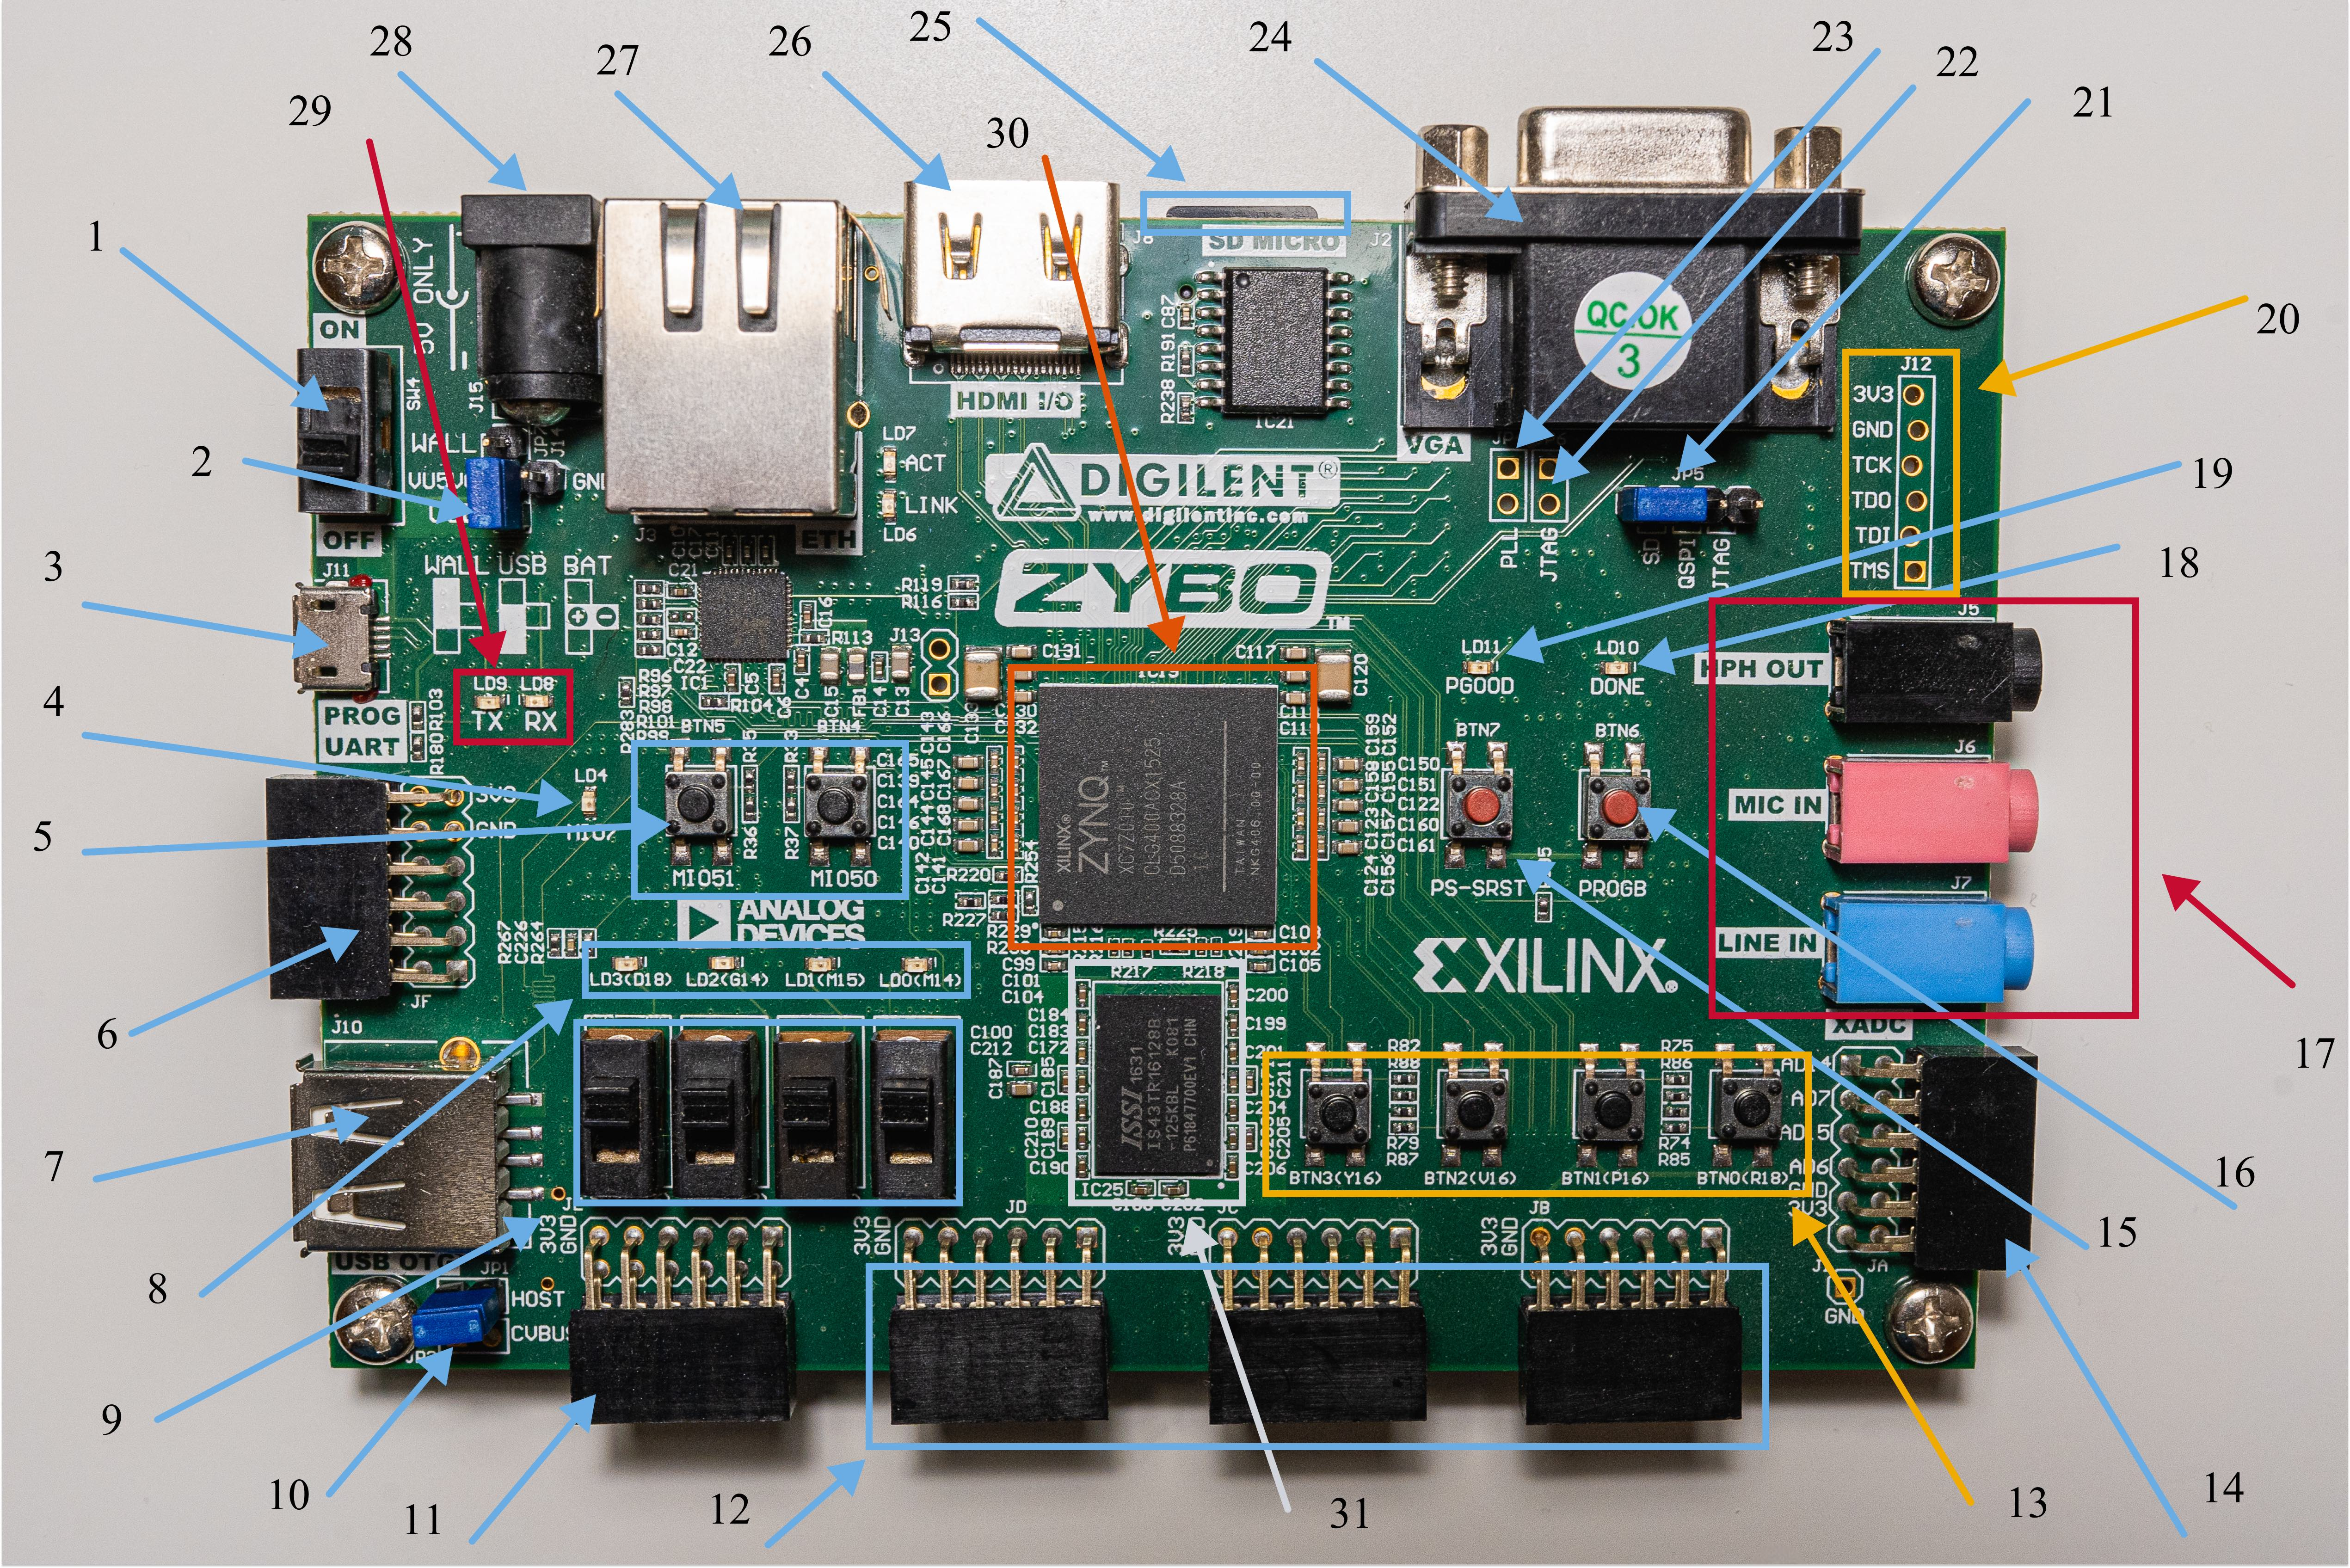
\includegraphics[width=1\textwidth]{src/jpg/digilent-zybo-foto-1-oznacene.jpg} 
						\caption{Vývojová deska Digilent ZYBO Zynq-7000 ARM/FPGA SoC Trainer Board vrchní pohled s vyznačením komponent.}
						\label{fig:digilent-zybo-foto-1-oznacene}
				\end{figure}

				\begin{figure}[H]
					\centering
						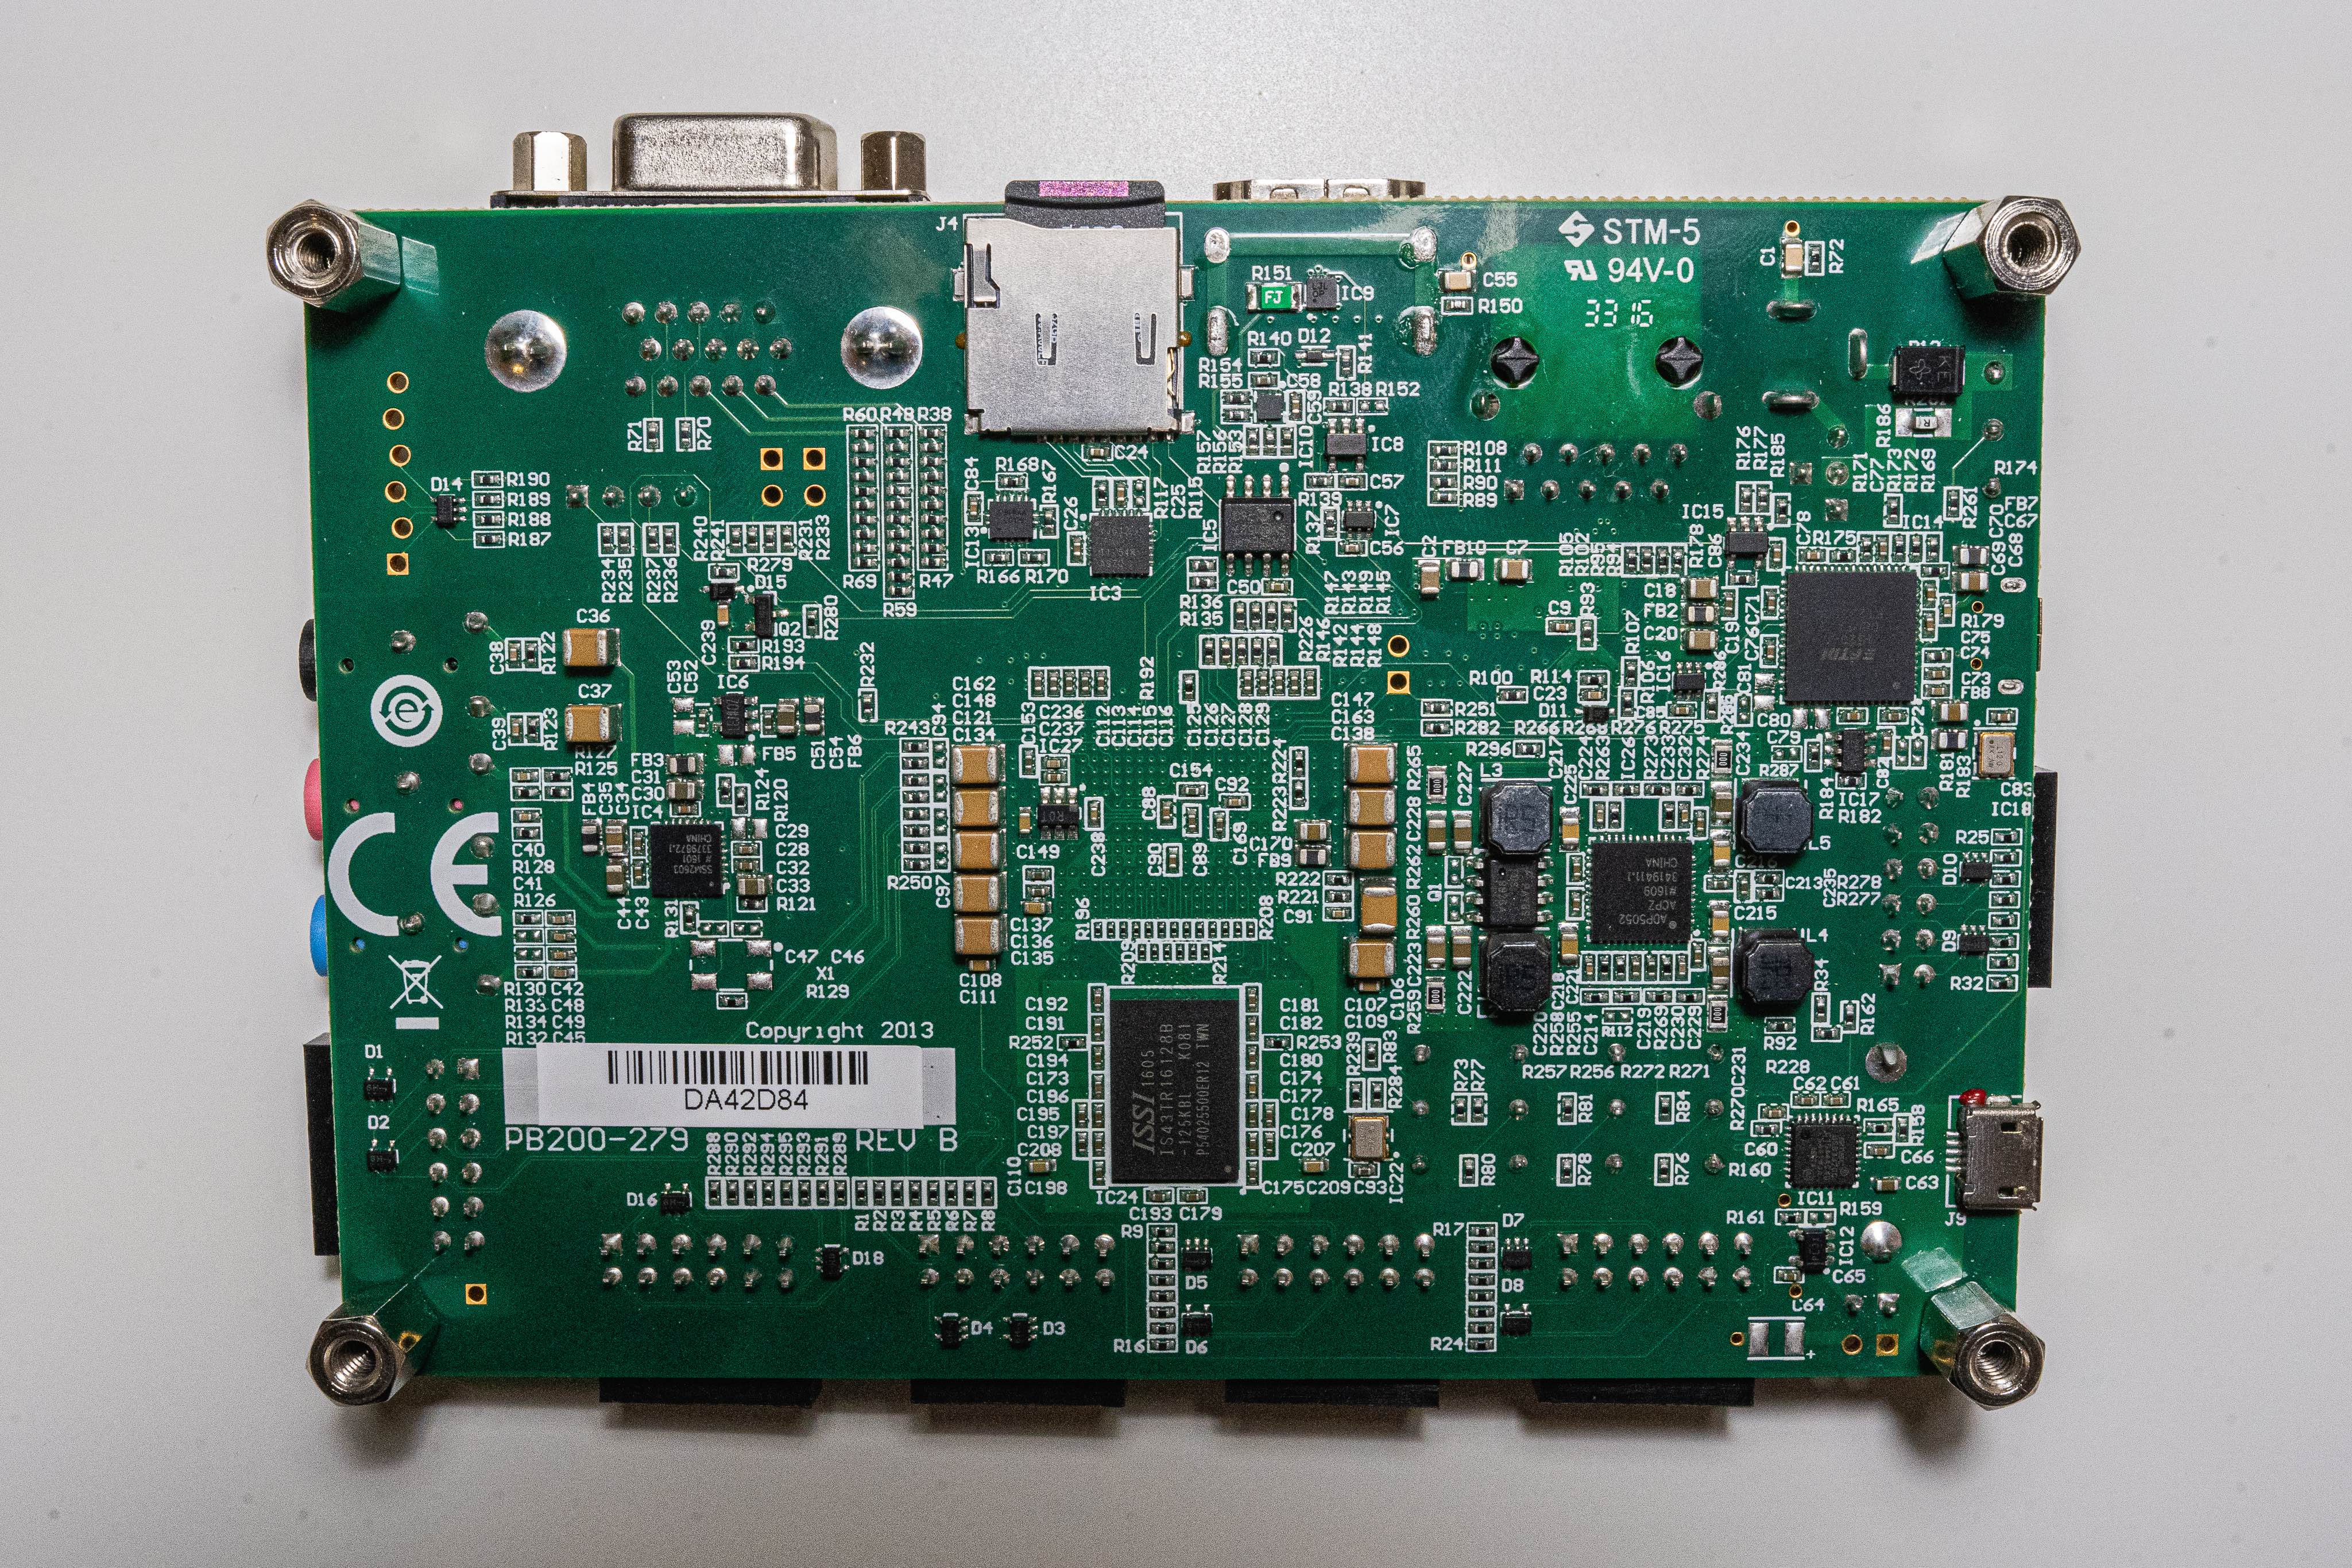
\includegraphics[width=1\textwidth]{src/jpg/digilent-zybo-foto-3.jpg} 
						\caption{Vývojová deska Digilent ZYBO Zynq-7000 ARM/FPGA SoC Trainer Board spodní pohled.}
						\label{fig:digilent-zybo-foto-3}
				\end{figure}

				\fbar
			\begin{table}[htbp!]
				\centering
				\caption{Popis označených komponent na vývojové desce Digilent Zybo Zynq-7000. (informace a značení z \cite{digilent-zybo-reference-manual})}
			  \vspace*{0.15cm}
			   \resizebox{\textwidth}{!}
				{
				\begin{tabular}{!{\vrule width 2pt} c | l | l !{\vrule width 2pt}}\noalign{\hrule height 2pt}
				označení & popis &	poznámka \\
				\noalign{\hrule height 2pt}
				1 & Power Switch & galvanické sepnutí napájecího obvodu \\ \hline
				2 & Power Select Jumper and Battery Header & výběr napájecího vstupu konektor, USB, baterie\\ \hline
				3 & Shared UART/JTAG USB port & komunikace UART a JTAG debugging\\ \hline
				4 & MIO LED & multiplexed LED – možnost výběru signálu\\ \hline
				5 & MIO Pushbuttons (2) & multiplexed input\\ \hline
				6 & MIO Pmod & možnost připojení periférií\\ \hline
				7 & USB OTG Connectors & USB port typ A/micro USB (spodní část)\\ \hline
				8 & Logic LEDs (4) & zobrazování 1/0\\ \hline
				9 & Logic Slide Switches (4) & logický vstup 1/0\\ \hline
				10 & USB OTG Host/Device Select Jumpers & výběr módu zařízení\\ \hline
				11 & Standard Pmod & chráněné Pmod, limitace max. přenosu informace\\ \hline
				12 & High-speed Pmods (3) & jako standard ale bez ochrany, vyšší rychlost\\ \hline
				13 & Logic Pushbuttons (4) & logický vstup 1/0\\ \hline
				14 & XADC Pmod & možnost  analog/digi input/output, spojeno s ADC v Zynq\\ \hline
				15 & Processor Reset Pushbutton & reset PL, paměti v PS\\ \hline
				16 & Logic Configuration reset Pushbutton & reset PL, zrušení DONE informace\\ \hline
				17 & Audio Codec Connectors & stereo line in, mono mikrofon, stereo output\\ \hline
				18 & Logic Configuration Done LED & signál o úspěšném dokončení konfigurace PL\\ \hline
				19 & Board Power Good LED & 1/0, 1 – nominální napětí na všech sběrnicích\\ \hline
				20 & JTAG Port for optional external cable & externí JTAG\\ \hline
				21 & Programming Mode Jumper & výběr „programovacího vstupu“, SD karta, QSPI, JTAG\\ \hline
				22 & Independent JTAG Mode Enable Jumper & JTAG mimo PS, viditelné pouze PL\\ \hline
				23 & PLL Bypass Jumper & přemostění PLL (CLK), pro možnost konfigurace PLL\\ \hline
				24 & VGA connector & připojení displaye\\ \hline
				25 & microSD connector & na spodní straně\\ \hline
				26 & HDMI Sink/Source Connector & input/ouput, nutné implementovat encoding a decoding v logice\\ \hline
				27 & Ethernet RJ45 Connector & komunikace\\ \hline
				28 & Power Jack & napájení 5 V/2,5 A\\ \hline
				29 & TX/RX LED & indikace UART komunikace\\ \hline
				30 & Xilinx Zynq SoC & srdce desky\\ \hline
				31 & DDR2 Memory & RAM\\\noalign{\hrule height 2pt}
				\end{tabular}
				}
				\label{tab:digilent-zybo-zynq-7000-description}
			\end{table}


			

		\fbar
		\subsection{Možné alternativy}
			% Novější verze Zybo
			% Něco jiného
			% Custom řešení - ZynQ Berry
			%  [ZynQBerry](https://shop.trenz-electronic.de/en/TE0726-03-11C64-A-ZynqBerry-Module-with-Xilinx-Z-7007S-Single-Core-Raspberry-Pi-2-compatible) (velice zajímavější i díky ceně, ale možná by hodně cool bylo celé si udělat sám sestavu)

\section{Matematický model stroje}
	\subsection{Představení stroje}
	\subsection{Odvození modelu}
	\subsection{Optimalizace modelu}

\section{Aplikace pro FPGA a CPU}
V této části jsou představeny jednotlivé nástroje, využívané při tvorbě programu pro CPU a akcelerované aplikace na FPGA. Je důležité zmínit, že na tzv „host“ (ARM procesor) je skutečně spuštěný řídící program akcelerované aplikace. Na PL (FPGA) je poté vytvořen HW, který reprezentuje myšlené algoritmy aplikace. Proto není korektně správné mluvit o tom, že se vytváří program pro FPGA. Proto v této práci bude používáno označení pro vytváření HW na PL vytváření „kernel“.\par
	Dále jsou v této části představeny postupy, které vedou k úspěšnému používání vývojových nástrojů. Poté je vysvětlena tvorba samostatné aplikace, která je hlavní náplní této práce.
	\subsection{Použité nástroje}
		Tvorba akcelerované aplikace může být obecně prováděna více způsoby. Tento způsob závisí na použitém vývojovém nástroji HW. V této práci je využíváno SoC od firmy Xilinx, proto je výhodné využívat již připravené nástroje, které umožní snazší vývoj SW, tvorbu HW a přípravu systému na SoC.\par
		Veškerý používaný SW v této práci od firmy Xilinx je po registraci volně dostupný ke stažení.\par
		Tato část představuje jednotlivé použité nástroje firmy Xilinx a nastiňuje postupy, které je třeba dodržet k úspěšnému zprovoznění a používání nástrojů.
		\subsubsection{Xilinx Vivado}\label{subsubsec:xilinx-vivado}
		\subsubsection{Xilinx Vitis}\label{subsubsec:xilinx-vitis}
		\subsubsection{PetaLinux}\label{subsubsec:petalinux}
		\subsubsection{Programovací prostředí – operační systém Linux}
			Pro práci s představenými vývojovými prostředími jako je \hyperref[subsubsec:xilinx-vivado]{Xilinx Vivado}, \hyperref[subsubsec:xilinx-vitis]{Xilinx Vitis} a \hyperref[subsubsec:petalinux]{PetaLinux} je nutné využívat podporovaných operačních systémů, které umožňují správnou funkci využitých nástrojů.\par
			Jednotlivé požadavky na operační systémy je možné nalézt na stránkách dokumentace \href{https://docs.xilinx.com}{\textcolor{ctublue}{https://docs.xilinx.com}}. Pro nejnovější verze v době zpracování této práce jsou požadavky pro \hyperref[subsubsec:xilinx-vivado]{Xilinx Vivado} dostupné v \cite{xilinx-vivado-design-suite-user-guide-2022}. Požadavky na operační systém pro \hyperref[subsubsec:xilinx-vitis]{Xilinx Vitis} v \cite{vitis-unified-software-platform-documentation-2022}. Pro využivání a tvorbu \hyperref[subsubsec:petalinux]{PetaLinux} je třeba dodržet systémové požadavky uvedené v \cite{petalinux-tools-documentation-2022}.
			Pokud uživatel využívá starších verzí vývojových nástrojů, je doporučováno využít operační systém Linux. Pro tuto práci bylo využíván systém Ubuntu 18.04 LTS (Bionic Beaver), dostupný ke stažení na adrese \href{http://old-releases.ubuntu.com}{\textcolor{ctublue}{http://old-releases.ubuntu.com}}. V průběhu práce došlo k aktualizování původních starších verzí SW a vešekrá práce byla přenesena na novější verzi systému Ubuntu 20.04 LTS (Focal Fossa).\par
			Je důležité poznamenta, že neplatí skutečnost, že když např. Vivado podporuje některou z novějších verzí Ubuntu, bude jí podporovat také PetaLinux. Vždy je doporučeno využívat starší verze a kontrolovat vzájemnou kompatibilitu, aby se předešlo zbytečné ztrátě času. Stahování SW, instalace a nastavování nástrojů je značně časově náročné.\par
			V případě využívání představených nástrojů a systému Linux je třeba dbát na správné postupy instalací a v případě problémů využívat dostupné dokumentace.
		% Jaké verze jsou momentálně podporované
		% Co je třeba nainstalovat za balíčky před započetím instalace
		% Jaký je flow aby byla možná příprava systému
		% Proč zrovna linux Open Source
	\subsection{Tvorba HW architektury Xilinx Vivado}
	% Basic popsání, možná si zjistit do hloubky co vše znamená
    % WorkFlow
    % Zjistit jak dát vstupem tlačítka a jak výstupy jako výstupy

	\subsection{Tvorba PetaLinux}
	\subsection{Tvorba SW pro CPU a FPGA}

\section{Představení pracoviště}
\section{Dosažené výsledky}


		
%závěr
\newpage
\addcontentsline{toc}{section}{\numberline{}Závěr} 
\section*{Závěr}
Aliquam dapibus leo velit, ultrices eleifend mi feugiat eget. Aliquam euismod facilisis turpis, nec lobortis libero aliquet sit amet. Aenean suscipit ante eget ipsum viverra hendrerit. Ut sed massa sed nisi tempus dapibus in eu enim. Nullam vitae odio laoreet, malesuada purus non, faucibus orci. Lorem ipsum dolor sit amet, consectetur adipiscing elit. Etiam eget odio quis enim laoreet imperdiet nec eu nunc. Maecenas ut consequat purus. Duis faucibus risus nec metus cursus placerat. Phasellus sapien justo, laoreet in pulvinar ut, maximus nec velit.\par
	

\flushbottom %vyčištění stránky

%konec závěru

\newpage
\printbibliography[title={{Literatura}}]	
\nocite{*}
\addcontentsline{toc}{section}{\numberline{}Literatura} %Added citations to TOC%
	\appendix
	\titleformat{\section}{\color{ctublue}\fontspec{Times New Roman}\fontsize{15}{15}\bfseries}{Příloha \thesection:}{2.1em}{}
	\begin{appendices}
	\section{Seznam symbolů a zkratek}
		\subsection{Seznam symbolů}
			\begin{description}
			\item $\vec{F}$ (N) \hspace*{\parindent} vektor síly
			
		\end{description}
	\subsection{Seznam zkratek}
		\begin{description}
			\item DCM \hspace*{\parindent} DC Master
			
		\end{description}
	\end{appendices}
\end{document}
